\documentclass[output=paper]{LSP/langsci}  
\author{Guylaine Brun-Trigaud, Tanguy Solliec, Jean Le Dû} 
\title{A new dialectometric approach applied to the Breton language} 
% \epigram{Change epigram in chapters/01.tex or remove it there }
\abstract{This paper presents a new dialectometric approach applied to the Breton language in the heart of the Breton-speaking Brittany. It is based on data culled in the Nouvel Atlas Linguistique de la Basse-Bretagne \cite{le_du_nouvel_2001}.

We process statistically qualitative data using the Levenshtein algorithm which allows us to accurately measure and take into account the discrepancies or similarities between different pronunciations of a given word. 

This contribution aims to determine whether linguistic distance is caused by a frequent repetition of the same phenomenon or whether it is the outcome of multiple changes. Our first results propose new ways of analysing Breton data.

}
\maketitle 
\begin{document}
 

% Guylaine Brun-Trigaud\\
% (CNRS \& Université de Nice-Sophia-Antipolis, France)
% 
% Tanguy Solliec\\
% (Université de Paris Descartes, France)
% 
% Jean Le Dû\\
% (Université de Bretagne Occidentale, France)

 

\section{Introduction}

At a time when the number of languages in use is bound to reduce drastically in the next decades, documenting endangered languages is a major challenge for linguists, as is the urgency to study and analyse their inner variations. Nowadays, Breton is considered to be as an endangered language, according to the definition proposed by UNESCO \citep{moseley_atlas_2010}. The intergenerational transmission of the language ceased during the 60’s. Most of its speakers are now over 70 years of age and, at present, the language is disappearing quickly. We propose to present a dialectometric approach applied to the Breton language based on Le Dû’s \textit{Nouvel Atlas Linguistique de la Basse-Bretagne} (henceforth NALBB) \cite{le_du_nouvel_2001} so as to re-examine the geolinguistic landscape of Lower Brittany.

Little dialectometric work has been done on the Breton language (\citealt{german_etude_1984}, \citealt{german_methode_1991}, \citealt{costaouec_linguistic_2012}). Our approach is based on a new methodology: we have implied the principles of the edit distance (\textit{i.e.} the Levenshtein algorithm, henceforth DL), which allows us to measure the linguistic distance between two strings of characters. This distance is defined as the minimal number of characters that need to be deleted, to inserted or to replaced, in order to transform one string of characters to another. We have introduced modifications in processing the data.

Our work was intended to test this new approach and to observe its advantages and disadvantages when applied to Breton. It was tested for the first time on dialects in the Occitan area. This research constitutes the very first step of a PhD thesis by \citet{solliec_dialectometrie_2014}, whose goal is to process the data available in the NALBB in order to sketch the geolinguistic configuration of the area based on a dialectometric approach. This first study focuses on the phonetics of Breton because the data contained in the NALBB are richer in phonetics than in the lexicon.

\section{Preliminary research}

\subsection[A first test on Occitan dialects]{A first test on Occitan dialects}

Dialectometry was initiated by \citet{seguy_relation_1971,seguy_dialectometrie_1973}, and \citet{guiter_atlas_1973}. Its aim is to quantify linguistic variation with the help of mathematical tools. This approach allows us not only to account for the differences or similarities between the dialects studied, but also to display them with the help of maps and tables. Nowadays, many research groups work with various methods. One of them, the Groningen School, led by Nerbonne and Heeringa (\citealt{nerbonne_computational_2001,nerbonne_measuring_2010}, \citealt{heeringa_measuring_2004}), uses the Levenshtein algorithm. This methodology allows for the accurate measurements of the number of operations (replacement, deletion or insertion) necessary to transform one string of characters to another and displays the results as a number or a percentage of similarity.

%%%
%%% Again a font/tipa error [OS]
%%%
\begin{table}
\begin{tabular}{llllllllll}
\lsptoprule
%Clermont (pt 22) & ʒ & u & r & ˈ & n & a & ð & ɔ & \\
%Fauillet (pt 20) & ʒ & u & ʀ & ˈ & n & a & d & œ & \\
&  &  & 1 &  &  &  & 1 & 1 & 3\\
\multicolumn{10}{l}{ 3 differences = 63\% of similarity / 37\% of dissimilarity}\\
\end{tabular}
\caption{An example of a quantitative measurement between 2 locations of enquiry for the word ‘a day (long)’ in the Occitan language.}
\end{table}

As this method is intended to provide an overall characterization, it accounts most of the time for dialectal distance from a quantitative point of view. However, it does not describe the results qualitatively in a direct way. In others words, it doesn’t indicate the exact proportion of each difference involved in dissimilarity. Does the dissimilarity result from one sole phoneme susceptible to massive variation while other kinds of variations remain very minor or, on the contrary, does the dissimilarity result from an important array of different variations which are more or less of equal importance? In the first case, mutual comprehension between the speakers is not really affected, while in the second case, it is likely to be jeopardized. In order to contrast the two kinds of variation, Brun-Trigaud decided to modify the algorithm. To accomplish this, she implemented it as a VBA function in an Excel spreadsheet so as to obtain, not a percentage or a number of characters, but rather the nature of the phonemes undergoing the operations. She then treated them statistically. She carried out a first experiment \citep{brun-trigaud_usage_2014} using data taken from the \textit{Atlas Linguistique et Ethnographique du Languedoc Occidental} \citep{ravier_atlas_1978}, a region located in the Occitan area in southern France. This language area is distinguished by both a large and relatively homogeneous central zone around the city of Toulouse and by two mixed zones, one to the North in contact with Limousin and the other to the South, bordering the Catalan-speaking area.

%%%
%%% more (t)ipa errors [OS]
%%%
\begin{table}
\begin{tabular}{lllllll}
\lsptoprule
segments & concept & answ (22) & answ (20) & DL1 & DL2 & DL3\\
%22 {\textgreater} 20 & { day} & { ʒurˈnaðɔ} & { ʒuʀˈnadœ} & { repl. r by ʀ} & { repl. ð by d} & repl. ɔ by œ\\
%22 {\textgreater} 20 & { he snores} & { ˈrː\~{u}ŋkɔ} & { ˈʀ\~{u}ŋklœ} & { repl. rː by ʀ} & { ins. of l} & repl. ɔ by œ\\
%22 {\textgreater} 20 & { fair} & { ˈfjɛrɔ} & { ˈfjɛʀɔ} & { repl. rː by ʀ} & { repl. ɔ by œ} & \\
\lspbottomrule
\end{tabular}
\caption{An example of a qualitative measurement between 2 locations of enquiry for Occitan}
\label{tab:2}
\end{table}

%%%
%%% more (t)ipa errors [OS]
%%%
When all the data taken from two different locations were compared, as in \tabref{tab:2}, she obtained: replacing {r} by 
%{ʀ} = 36\% and replacing {ɔ} by {œ} = 22\%. 
Brun-Trigaud demonstrated that, for the area studied, from East to West, divergences were caused by the preponderance of only one phonetic variation, appearing in a massive way whereas in the North of the area differences appear in numerous phonetic variables which affects mutual understanding between speakers of different areas.

In order to validate these initial results, she invited her fellow Breton dialectologists, Solliec and Le Dû, the author of the NALBB, to test the new version of the algorithm on Breton data.

\section[Earlier dialectometric works on Breton ]{Earlier dialectometric works on Breton }
  
\begin{figure}
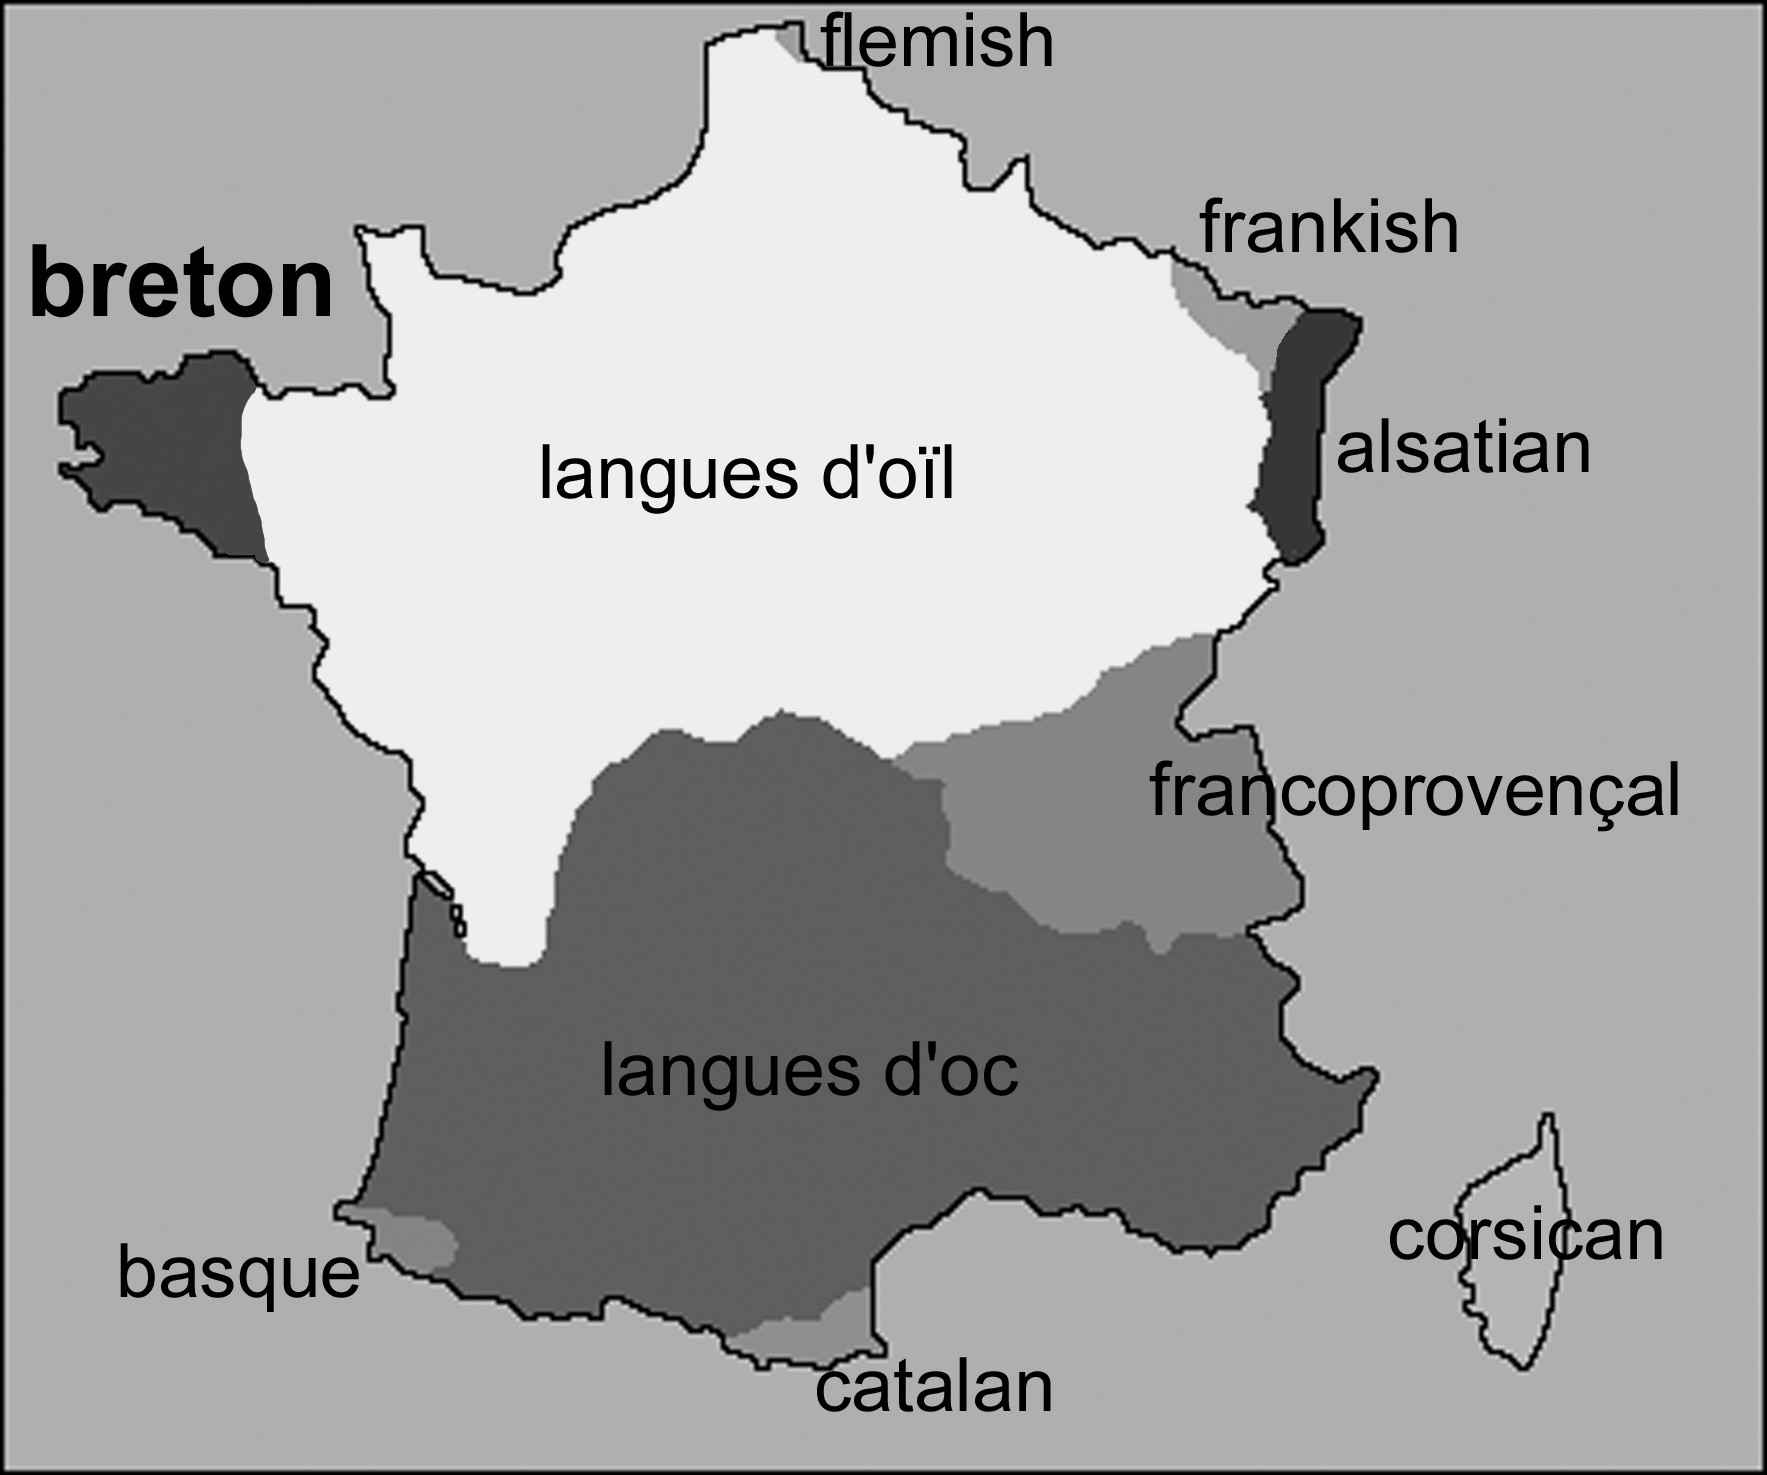
\includegraphics[width=\textwidth]{illustrations/brun_etal_fig1}
\caption{Situation of the Breton language.}
\label{fig:1}
\end{figure}

Works by \citet{falchun_perspectives_1981} based on the \textit{Atlas Linguistique de la Basse-Bretagne} (\citealt{le_roux_atlas_1924}, henceforth ALBB) have deepened the geolinguistic understanding of the Breton language. They constitute an important reference on the issue. 

Until now very little quantitative work has been applied to the description of the Breton language. \citet{german_etude_1984,german_methode_1991} is the very first to have applied a dialectometric approach to Breton data. A cluster analysis using the Lerman algorithm allowed him to classify the dialect areas according to their linguistic similarities and differences with the Breton of Saint-Yvi he described in his PhD thesis (\citeyear{german_etude_1984}). More recently \citet{costaouec_linguistic_2012} correlated the internal dialect borders inside a small area of the Breton speaking region with other aspects of social, cultural or economical factors around the village of La Forêt-Fouesnant whose dialect he described in his thesis \citet{costaouec_breton_1998}. These two studies are based on Le Roux’s ALBB whose data were collected between 1913 and 1920 for a range of 87 points of enquiry published in 600 maps. Le Dû began working on his NALBB (\citeyear{le_du_nouvel_2001}) in 1968 (187 points and 601 maps). He himself transcribed all the data in order to avoid transcription biases. Since no recent study has tackled the Breton language as a whole, as we have mentioned before, further works by Solliec will aim to fill in the gap. In order to accomplish this, he will take into account the NALBB data. This article constitutes the very first step in this process.

\section{The area investigated}

\begin{figure}
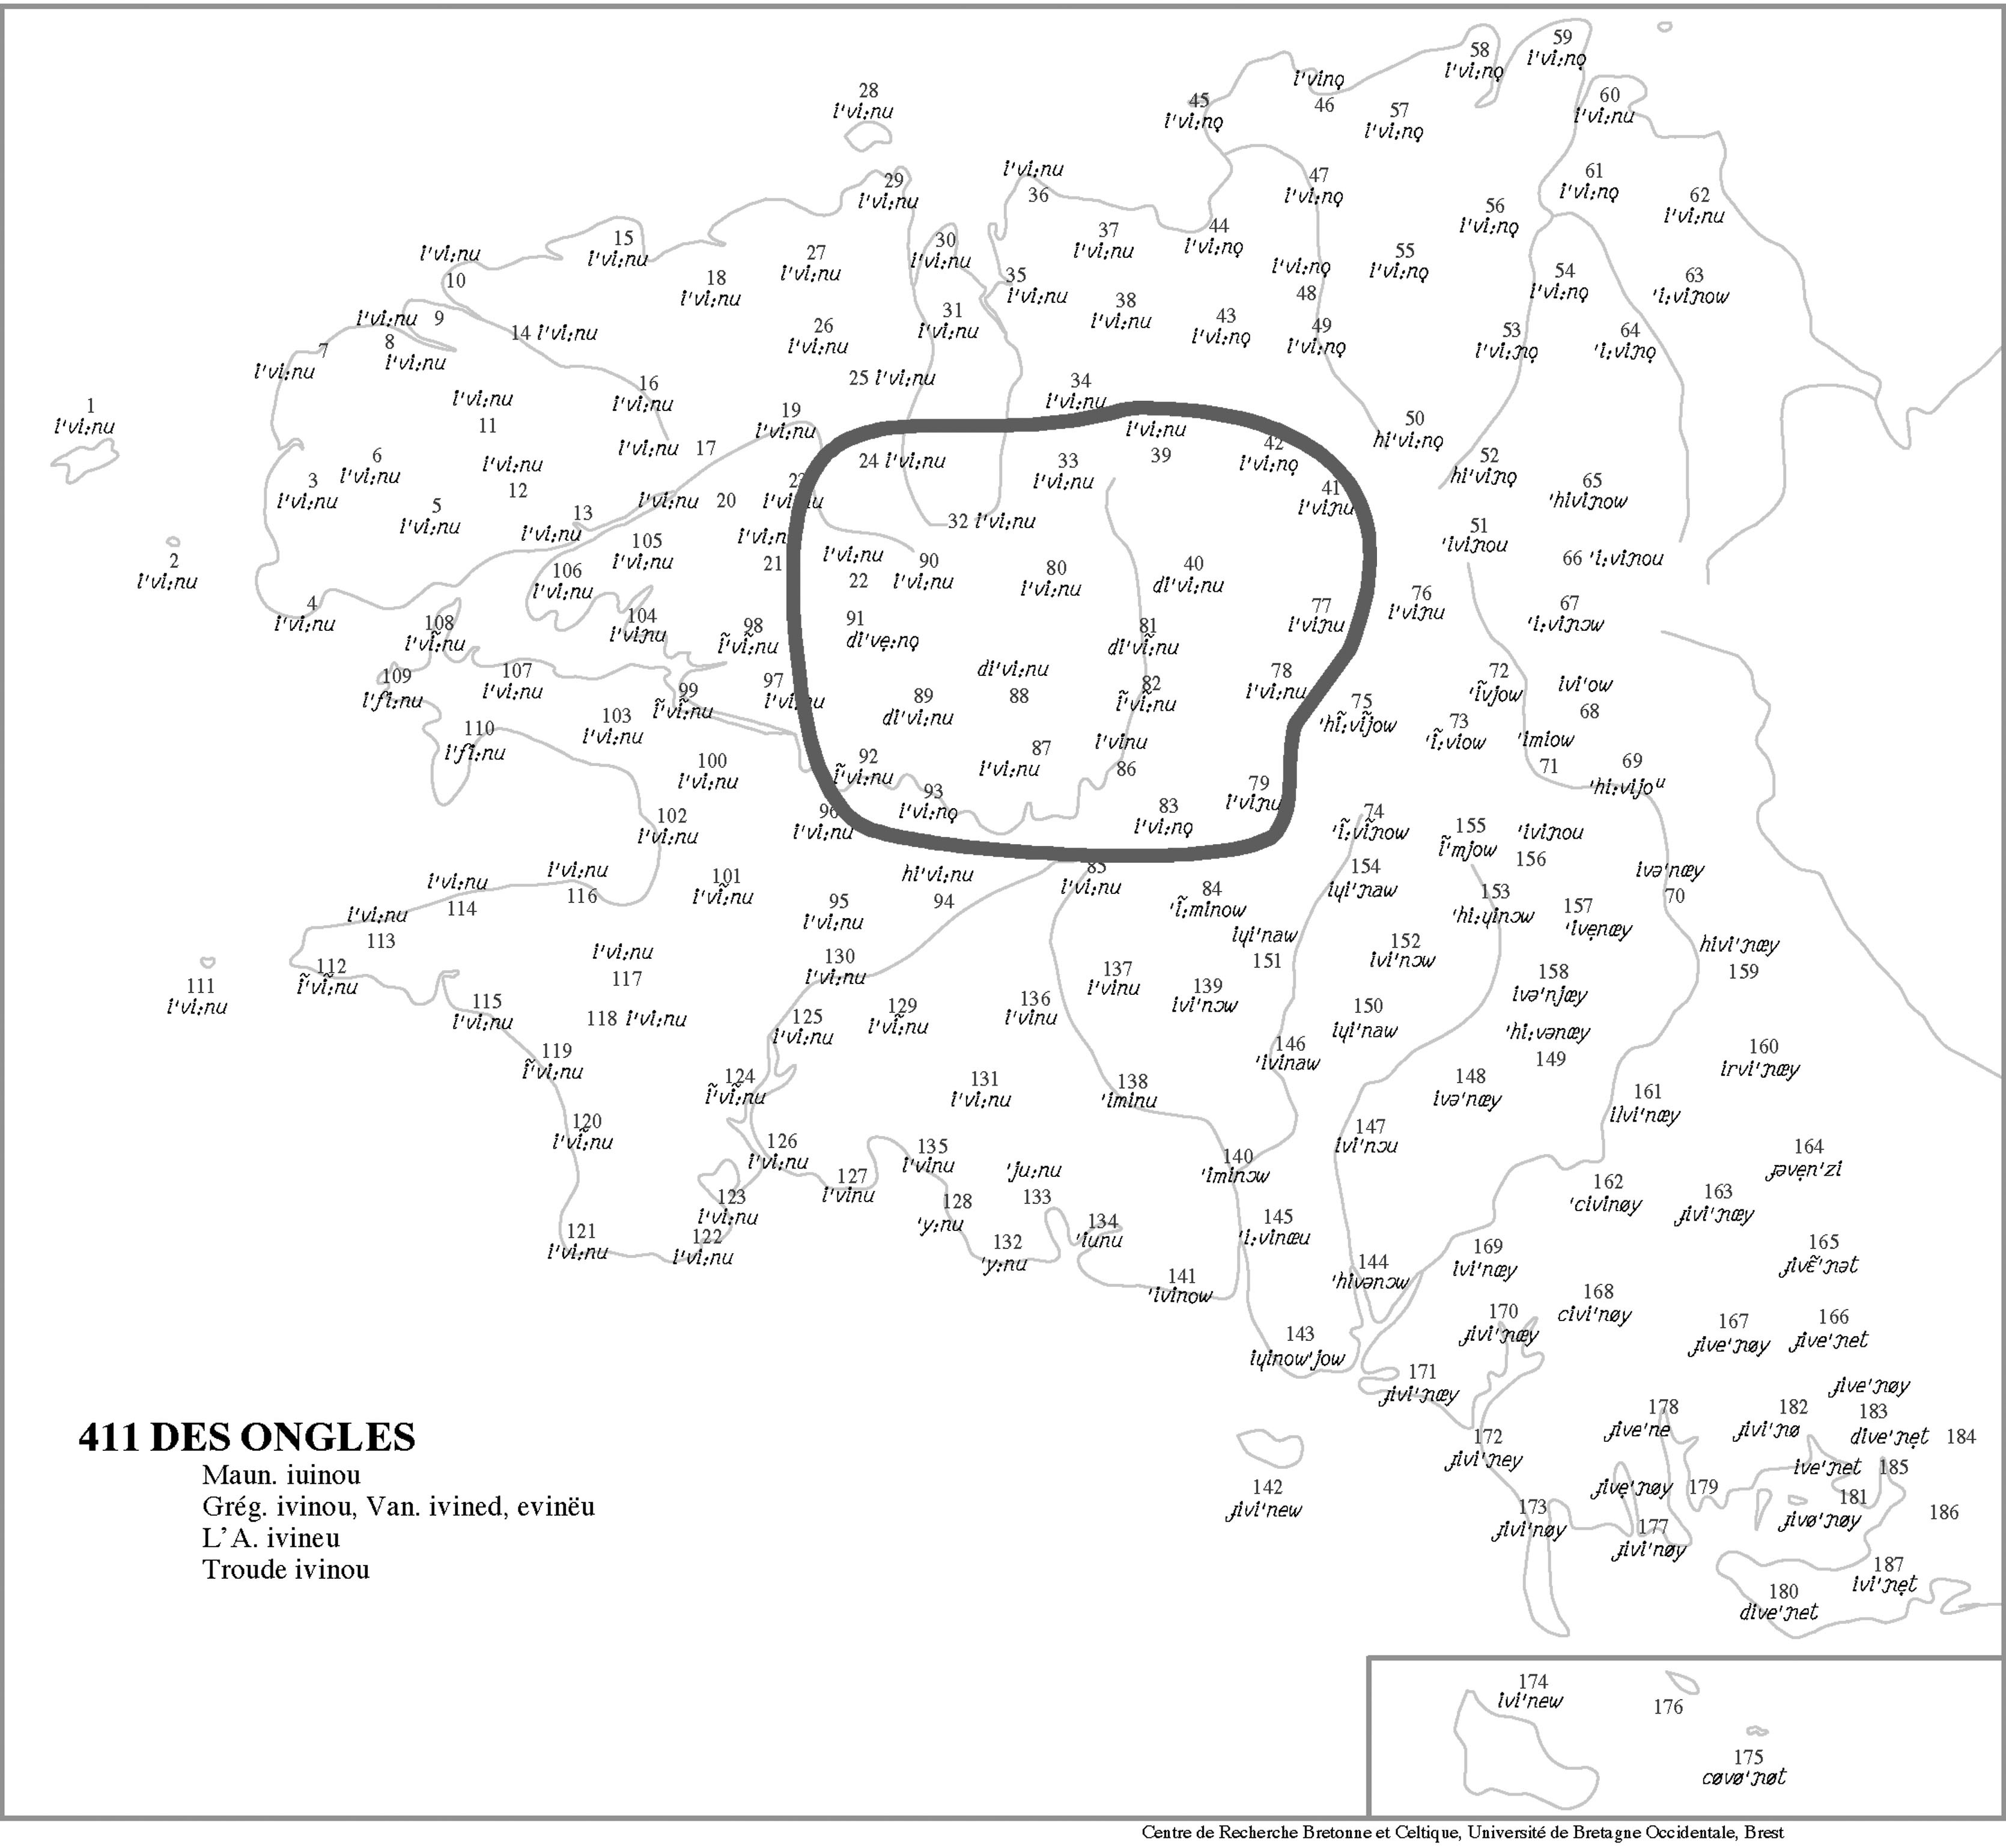
\includegraphics[width=\textwidth]{illustrations/brun_etal_fig2}
\caption{NALBB Map 411 ‘Fingernails’. The area investigated is delimited in black.}
\end{figure}
%\textit{\figref{fig:2}}: NALBB Map 411 ‘Fingernails’. The area investigated is delimited in black

We have willingly chosen to investigate a restricted and quite homogeneous area for the following reasons: on the one hand, we do not want to confront this modified version of the DL algorithm, from a technical point of view, with an area where linguistic variation is very intense, as in the case of the \textit{Vannetais} dialect (South-East of Lower-Brittany). Moreover, as was shown by \citet{falchun_perspectives_1981}, innovations have been spreading across this region for centuries. It would then be interesting to compare them with points from more conservative peripheral areas. Over the past few years, Solliec has been carrying out a project to describe and document local varieties in this area and is therefore aware of the local variation phenomena.

On the methodological side, we have decided to use an interpoint approach: to do so, each location of the area is linked to its closest geographical neighbours in order to establish a comparison called the ‘segment’. Doing so allows the researcher to detect spatial continuities and geolinguistic breaches on a phonetic level \citep[137]{goebl_introduction_2012}. In this view we selected 23 investigation points for 165 phonetic maps (i.e. figuring only one lexeme and its different phonetic variations for each notion). We had not beforehand determined variables to observe in our corpus: our objective was to consider the data as a whole and to observe which phenomena produce linguistic distance and with which frequency.

It led us to divide the area into a net of 53 ‘segments’, which spatially connect each point on the atlas with its neighbours on the periphery. This brings us to a total of 8745 comparisons between strings of characters.

One of our first aims has been on the one hand to gather quantitative indicators and, on the other hand, to identify qualitatively the most recurrent facts involved in phonetic variation. Even though the latter are well known \citep{falchun_perspectives_1981,jackson_historical_1967}, we don’t know how frequently they occur.

\section{The problems DL meets with Breton}

In confronting DL with Breton language data, we noticed difficulties: \tabref{tab:3} shows an excerpt of the data where the algorithm repeatedly failed to analyze the data, while at the same time the FuzzyMatch function did not work as we can see in \tabref{tab:3}. This last function gives a percentage as a probability of correspondences.

\begin{table}
\resizebox{\textwidth}{!}{
\begin{tabular}{lllllp{0.25\textwidth}p{0.25\textwidth}p{0.25\textwidth}p{0.25\textwidth}}
\lsptoprule
segments & answ1 & answ2 & test Exact & FuzzyMatch & Levenshtein1 & Levenshtein 2 & Levenshtein 3 & Levenshtein 4\\
\midrule
40 {\textgreater} 41 & { h\~{e}̝:s} & { h\~{e}̝:s} & TRUE & Not a match &  &  &  & \\
32 {\textgreater} 80 & { 'e̝nes} & { 'e̝nnəs} & FALSE & 50\% (2) & { Rep. n by nn} & { Rep. e by ə} &  & \\
\hhline{~~~~~---~}
32 {\textgreater} 33 & { 'e̝nes} & { 'he̝nnəs} & FALSE & {25\% (3)} & {\textbf{\#VALUE! (Ins. of h)}} & {\textbf{\#VALUE! (Rep. n by nn)}} & {\textbf{\#VALUE! (Rep. e by ə)}} & \\
\hhline{~~~-----~}
33 {\textgreater} 39 & { 'he̝nnəs} & {{ h\~{e}̝:}} & {\textbf{FALSE}} & {\textbf{Not a match}} & Del. of s & Del. of ə & Del. of nn & {Rep. [1EB9?] by [1EB9?]}\\
\hhline{~~~--~~~~}
\lspbottomrule
\end{tabular}
}
\caption{Examples of the difficulties encountered by DL for the concept 'that one (masc.)'}
\label{tab:3}
\end{table}

Although we were careful to use a unique character for each phonetic segment and its diacritics, as is the case with diphthongs and geminates, it appears that the Levenshtein algorithm experiences difficulties when treating languages like Breton for which variation in the number of syllables is frequent (e.g., point 80 Berrien ['par[1ECD?]s] vs. point 81 Poullaouen [pa:ʀs] ‘parish’ (NALBB map 7)).

Nevertheless, after checking and adjusting the function, we ended by incorporating most observations. On the one hand, the raw results obtained from the FuzzyMatch function produces the following distribution (see map in \figref{fig:3}):

\begin{figure}
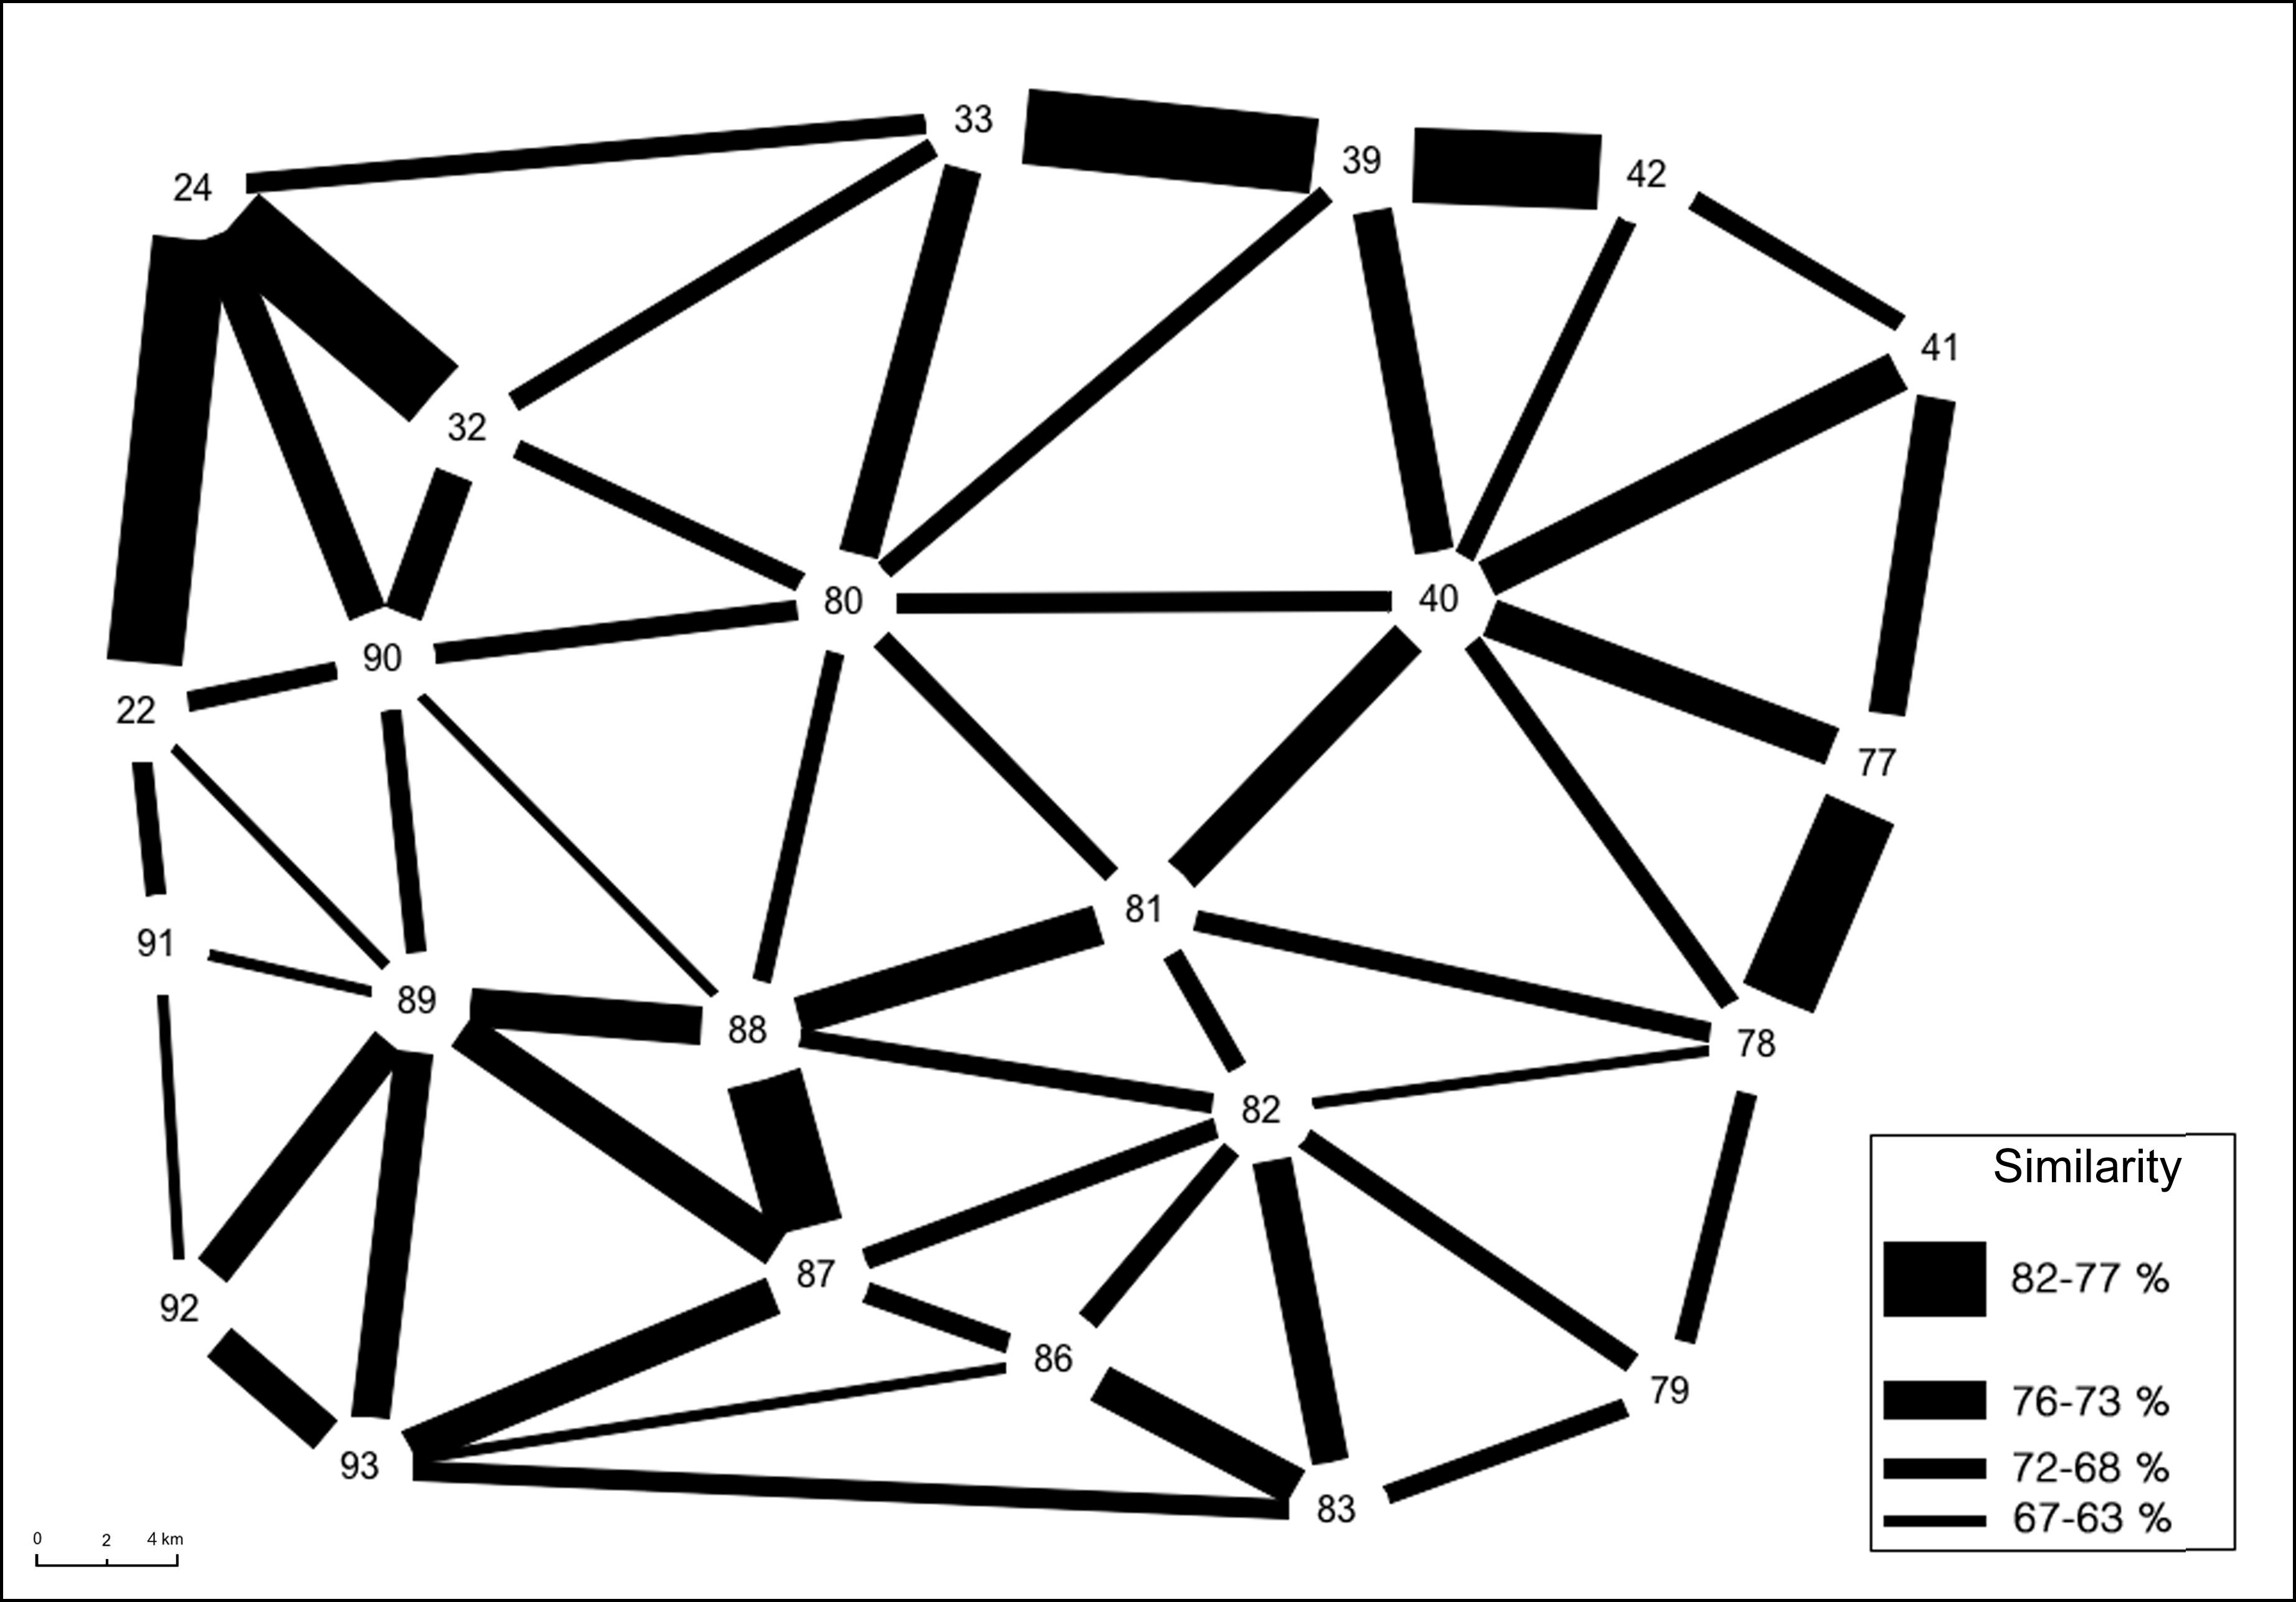
\includegraphics[width=\textwidth]{illustrations/brun_etal_fig3}
\caption{\textup{FuzzyMatch results for the area on a schematic map}}
\label{fig:3}
\end{figure}

The map shows several areas involving significant degrees of similarity, particularly in the North around points 24 on the one hand and 39 on the other, and in the South around point 88. It is clear that the geographic distance between the surveyed localities often correlates with phonetic similarity; for example, there is high phonetic similarity between nearby points 87 and 88 and low similarity between distant points 83 and 93. However, there are some exceptions, for instance, between points 22 and 24 or, vice versa, between 91 and 89. We will later see the reason why they occurred.

On the other hand, the results returned by the new function of the algorithm bring us to the following conclusions: first of all, amongst the 11,949 non-identical phonetic correspondences, ‘alternations’ or ‘differences’ according to our terminology, we had to manage an important dispersion of the distinctive correspondences (nearly 450). They were generated by the narrow phonetic transcription. With the consent of Le Dû, the author of the atlas, we grouped some alternations in order to have to deal with fewer details. This limited to 200 the number of the different kinds of alternations. The most frequent ones are listed in \tabref{tab:4}:

%%%
%%% fix table colours or think of alternative
%%%
\begin{table}
\begin{tabular}{lllll}
\lsptoprule
\hhline{~-~~~}
{ 1

} & { r/ʀ/ʁ

} & 14.70\% & 25\% & 50\%\\
\hhline{~-~~~}
 2 & e ([1EB9?]/e/eː) & 6\% &  & \\
 3 & a/ə & 4.5\% &  & \\
 4 & r (+/-) & 4.3\% & 25\% & \\
\hhline{~-~~~}
 5 & e/ə & 4\% &  & \\
\hhline{~-~~~}
 6 & ə (+/-) & 3.5\% &  & \\
 7 & e/ɛ & 3\% &  & \\
 8 & o ([1ECD?]/o/oː) & 3\% &  & \\
 9 & e/i & 2\% &  & \\
 10 & n (n/nn/ n̩) & 2\% &  & \\
 11 & æ/a & 1.7\% &  & \\
 12 & i (i/iː) & 1.6\% &  & \\
\lspbottomrule
\end{tabular}
\caption{List of the most frequent alternations}
\label{tab:4}
\end{table}

These alternations are distributed as follows on the following map (\figref{fig:4}): each segment (i.e. a pair of enquiry locations) is calculated according to the most frequent alternation proportionally to its frequency (perfect similarities are excluded).

  
%%please move the includegraphics inside the {figure} environment
%%\includegraphics[width=\textwidth]{BrunTrigaudLeDuSolliecfinal-img4.jpg}
\begin{figure}
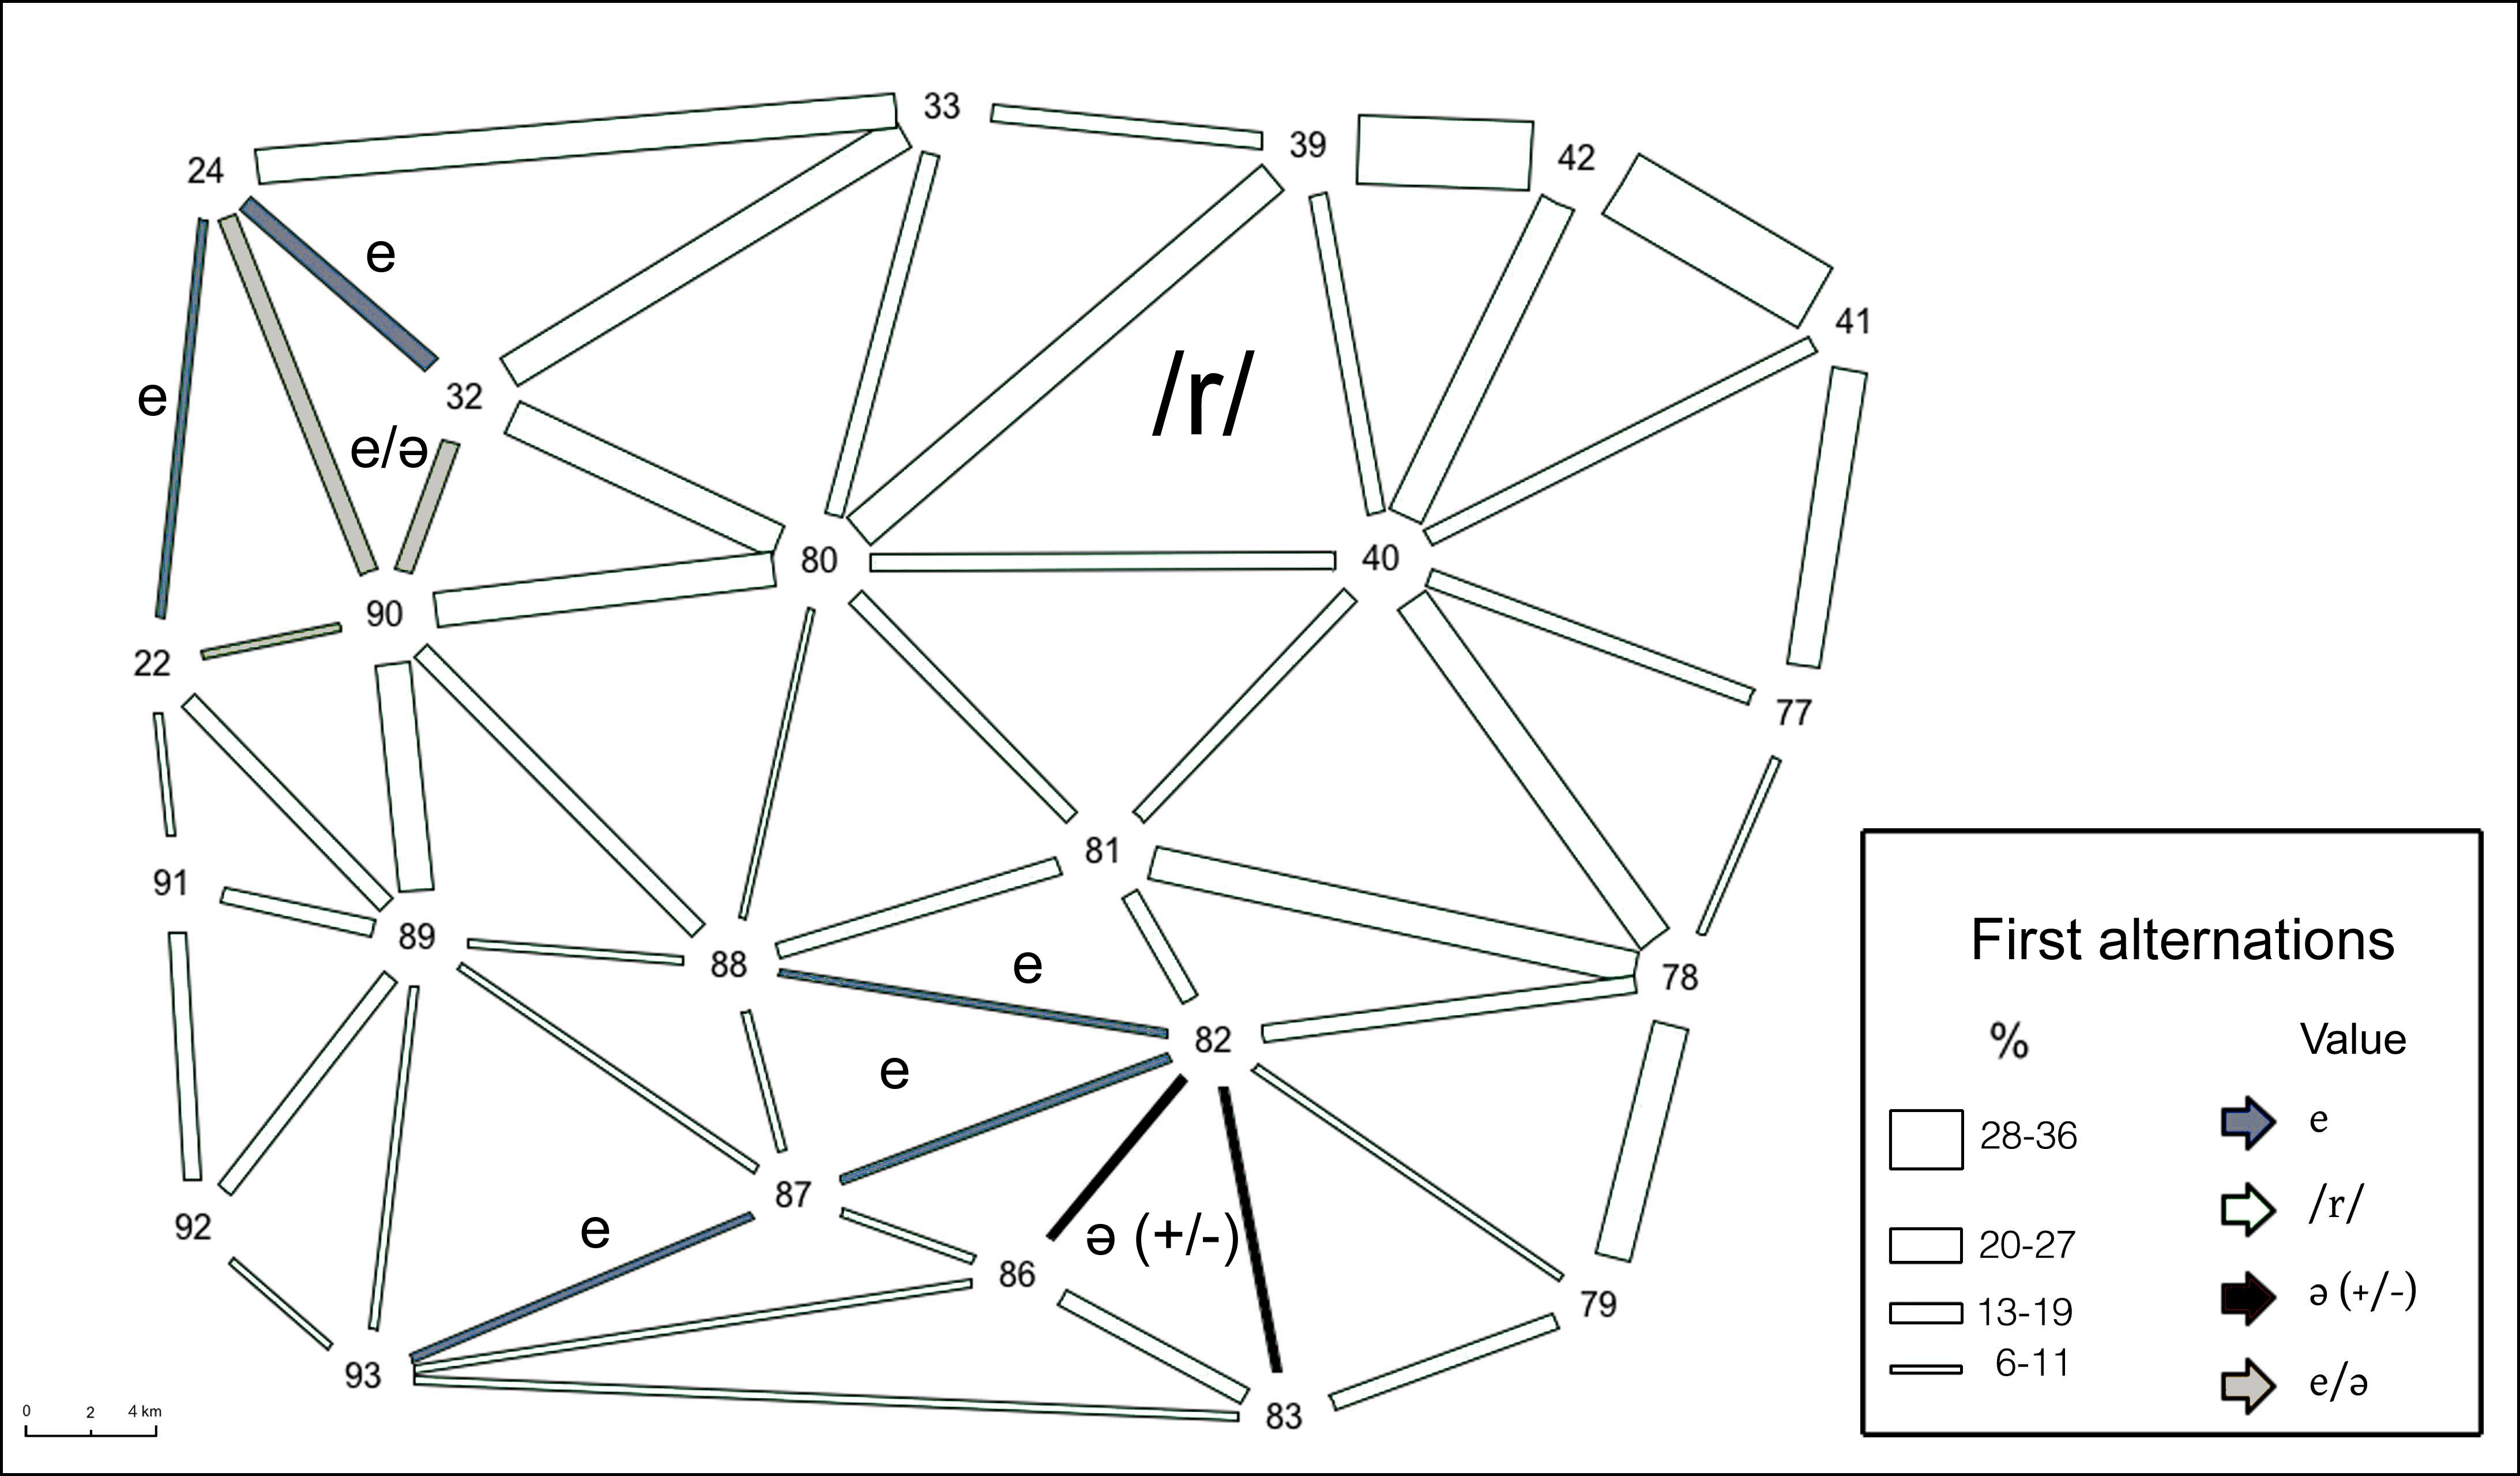
\includegraphics[width=\textwidth]{illustrations/brun_etal_fig4}
\caption{Distribution of the most frequent alternations across the area}
\label{fig:4}
\end{figure}

Apart from the [r] variations, the proportions of changes are relatively small, but they are quite similar to the results found in the Occitan region, with one notable difference: there were far more changes in the consonants \cite[135]{brun-trigaud_usage_2014}. In addition, as noted by Le Dû, [r] variations are probably idiolectal, so that we consequently decided to concentrate on other more relevant changes with his agreement.

The nature of the differences is more varied in the second most frequent alternation (map in \figref{fig:5}).

\begin{figure}
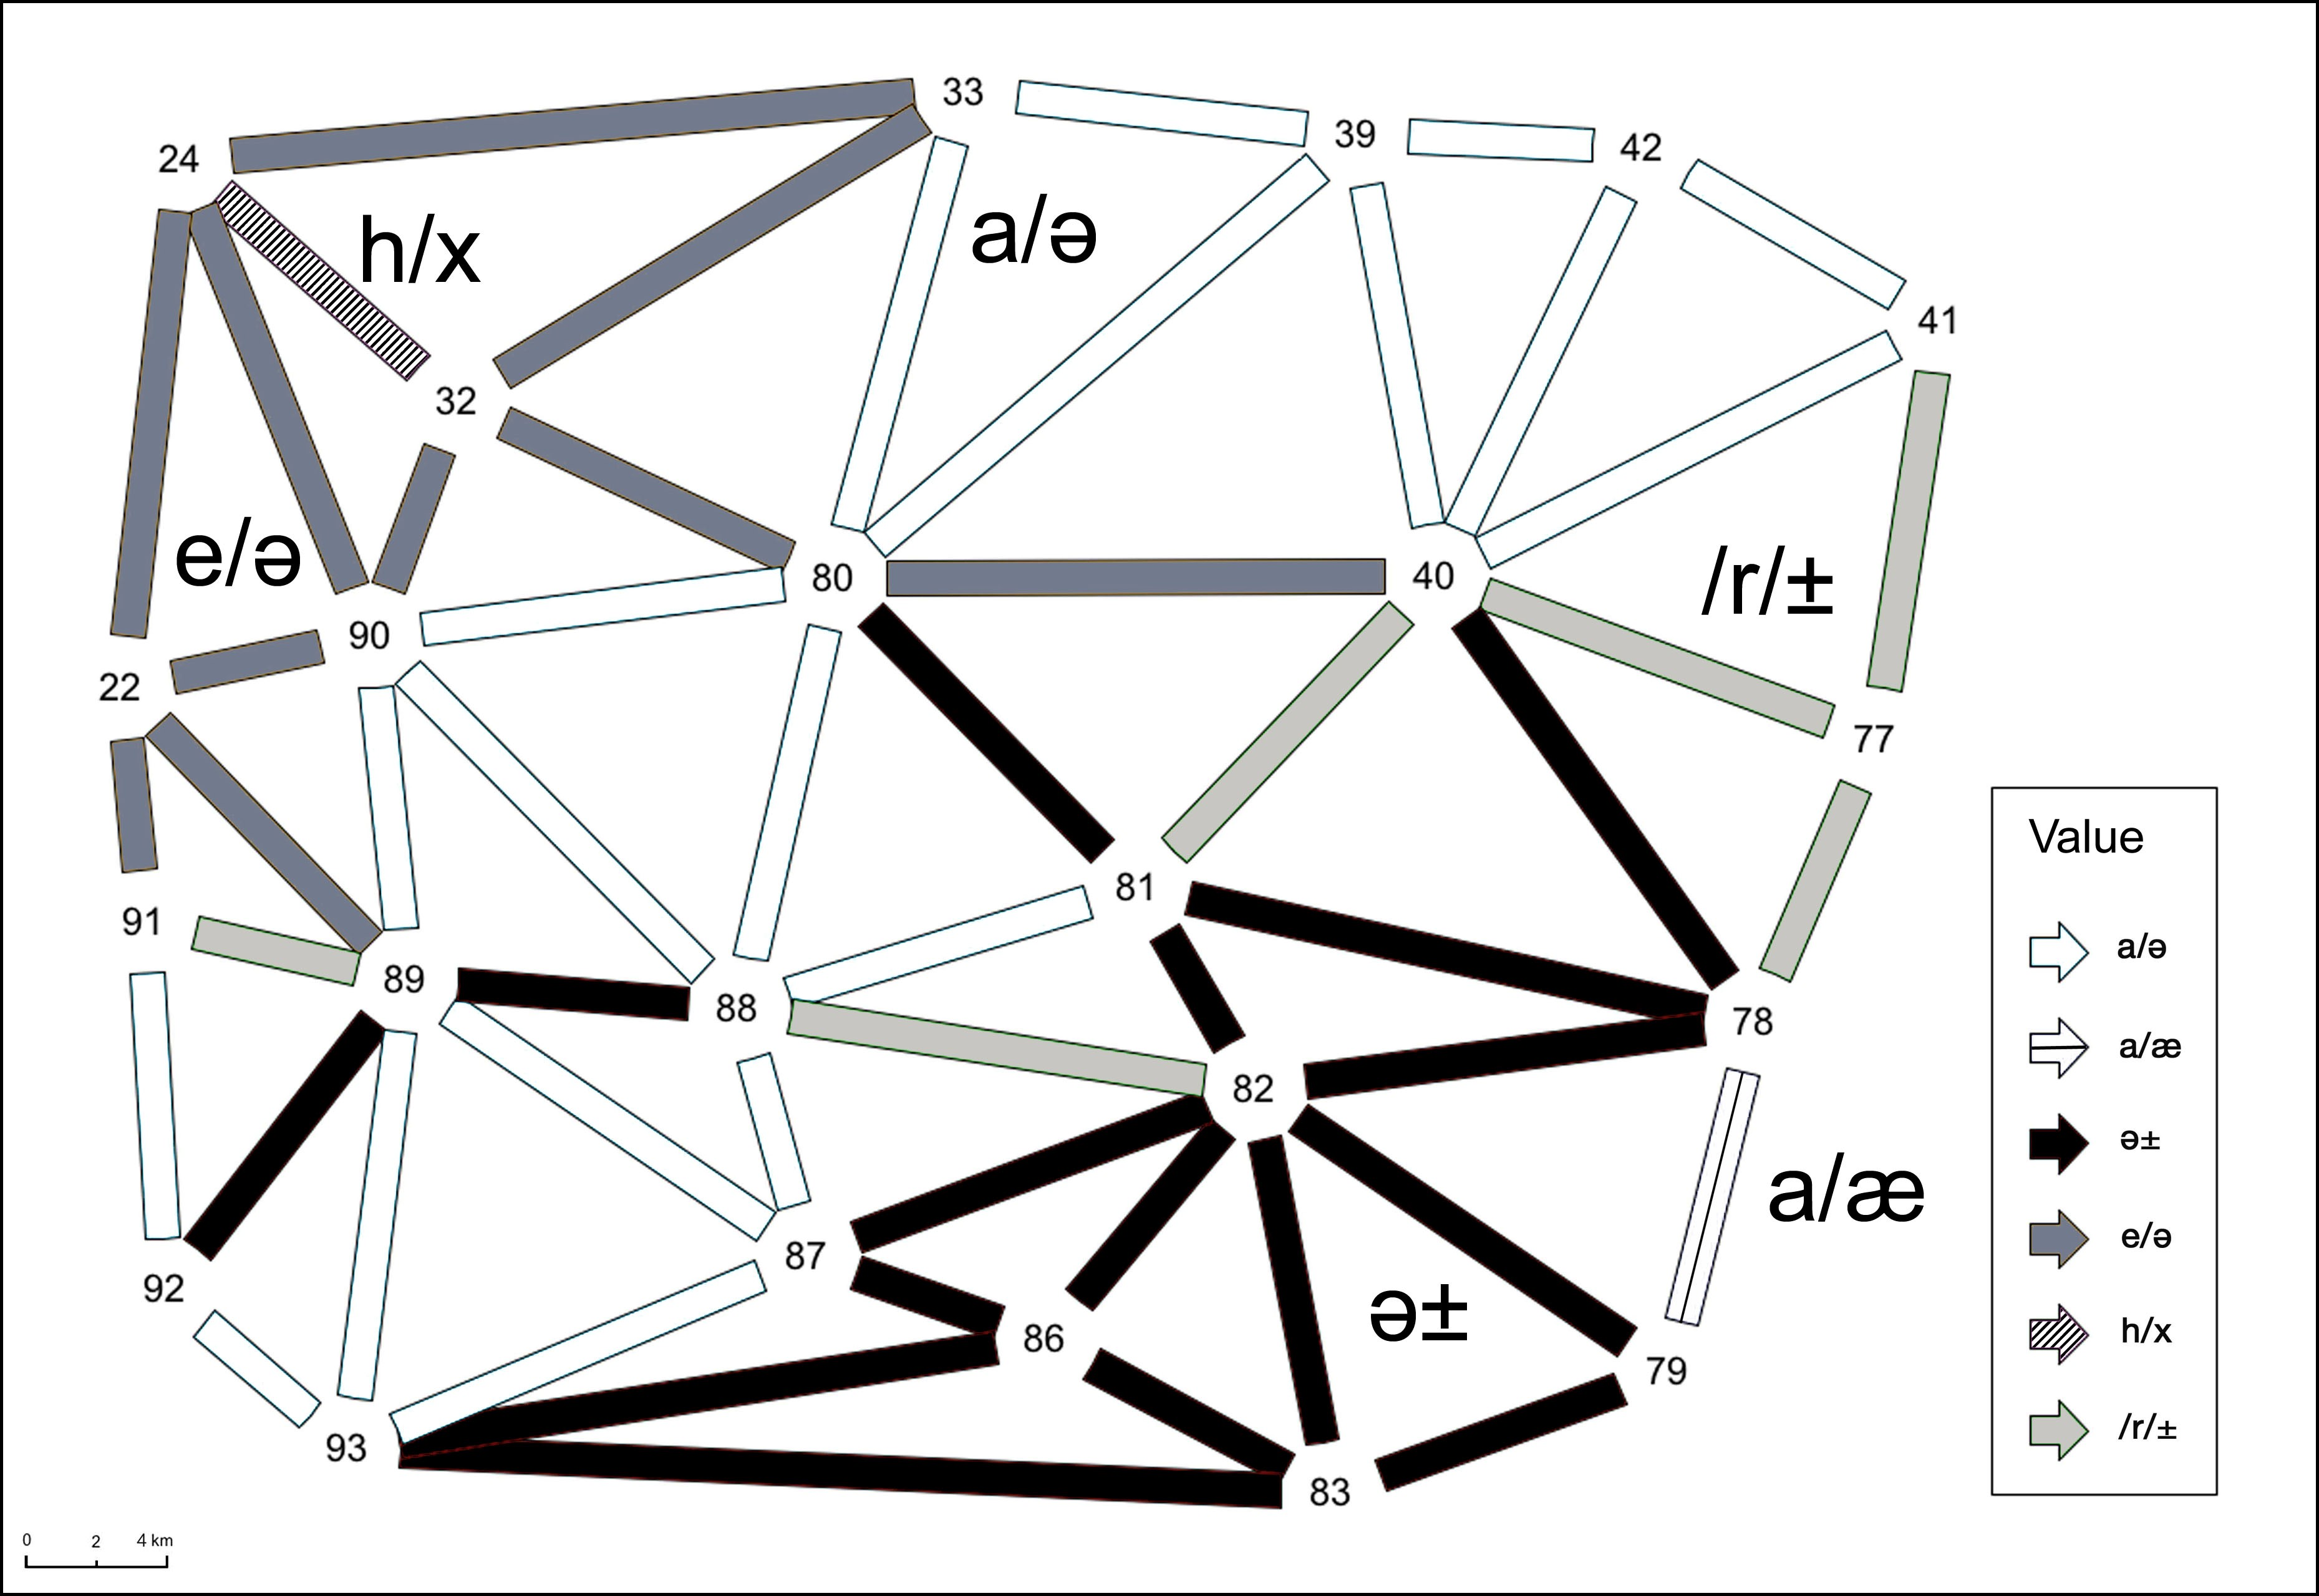
\includegraphics[width=\textwidth]{illustrations/brun_etal_fig5}
\caption{\textup{Distribution of the second most frequent alternation across the area}}
\label{fig:5}
\end{figure}

Taking into account the fact that the proportions of changes are relatively low – 3 to 13\% at most — the map in \figref{fig:5} shows that the south-eastern area is marked by the presence or absence of schwa (dark colour), the central area by alternations between [a] and [ə] (white colour), and, finally, that the north-west is characterized by an alternation between [e] and [ə] (dark grey).

\section{Analysing the first results }

The values the algorithm returned provided a considerable amount of data. They had to be explored carefully. The following analyses are instances of what can be done when scrutinizing geolinguistic data from a statistical perspective when associated with a qualitative approach. First, we will observe how one specific alternation occurs across the area, involving [a] and [ə]. Secondly, we will study the results for one locality, Collorec, point 88 of the NALBB.

\subsection[Examining only one kind of difference across the area ]{Examining only one kind of difference across the area }

The most important kind of change from a numerical point of view, apart from the variation of the rhotics, is the one which affects the vowels [a] and [ə]. In our corpus, this alternation ([a]/[ə])\footnote{ The alternation is indicated by the brackets ( ) in order to distinguish it apart from the specific sounds [a] and [ə]} constitutes 9\% of the non-identical phonetic correspondences we have gathered and appears in 54 of the 165 maps we selected.

The realizations [a] or [ə] occur in the following phonetic contexts. Each one can interplay with another:

%%%
%%% too wide
%%%
\begin{table}
\resizebox{\textwidth}{!}{
\begin{tabular}{p{.3\textwidth}p{.3\textwidth}p{.4\textwidth}}
\lsptoprule
 Type of context & Map number \& concept & Examples\\
a. Definite article’s initial vowel & 263 ‘the stable’ & (81) Poullaouen [ə hʀow] vs. (80) Berrien [a hʀow]\\
b. Final unstressed syllables & 464 ‘clothes’ & (93) Lennon ['diʎət] vs. (89) Lannédern ['diʎat]\\
c. Cluster of phones /-uwar/ or /-uarn/ & 196 ‘blackberries’ & (87) Landeleau ['mu:wəʀ] vs. (93) Lennon ['muwaʁ]\\
& 170 ‘iron’ & (32) Plounéour-Ménez ['u:aʁn] vs. (33) Plougonven ['u:ʀən]\\
d. Epenthesis vowel & 301 ‘(a) scythe’

(literary form: [falx]) & (78) Locarn ['valax] vs. (82) Plounévézel ['vʰaləx]\\
e. Infinitive mark & 50 ‘to count’ & (90) Botmeur ['k[1ECD?]ntə] vs. (32) Plounéour-Ménez ['k[1ECD?]nta]\\
\lspbottomrule
\end{tabular}
}
\caption{Phonetic contexts for the alternations ([a]/[ə])}
\label{tab:5}
\end{table}

Eighteen of the 165 maps we used included a definite article and 11 had infinitive word forms. These are instances of the alternations under study (see examples a and e in \tabref{tab:5}).

This strong presence may result from our selection of maps but, on the other hand, these alternations are very frequent in this language. On a more general level, ([a]/[ə]) alternation is interesting because it offers a perspective on the degree of centralization of vowels by Breton speakers. Breton final-syllable vowels tend to be centralized, when unstressed, especially in the central dialect area \citep[8-10]{wmffre_central_1998}. The occasional appearance of a clear [a] in post-stress context goes against the general economy of the language \citep{martinet_economie_1955}.

The ([a]/[ə]) alternation occurs regularly but with only a slight number of occurrences across the area. The data for this alternation can be classified according to their frequency of appearance in each location under enquiry. Three zones can be spotted according to the spatial distribution of the difference under examination (see \tabref{tab:6} and \figref{fig:6}). 

\begin{table}
\resizebox{\textwidth}{!}{
\begin{tabular}{lllll}
\lsptoprule
\begin{minipage}[t]{0.15\textwidth}N° of the location \end{minipage} & 
\begin{minipage}[t]{0.18\textwidth}Name of the location \end{minipage} & 
\begin{minipage}[t]{0.18\textwidth}Number of occurrences for the alternation ([a]/[ə]) \end{minipage} & 
\begin{minipage}[t]{0.18\textwidth}Proportion amongst these category of alternation (\%) \end{minipage} & 
\begin{minipage}[t]{0.18\textwidth}Proportion of the [ə] words involved in the alternation (\%) \end{minipage}\\
\midrule
 080 & Berrien & 93 & 8.80 & 65.6\\
 090 & Botmeur & 80 & 7.57 & 46.25\\
 040 & Plourac’h & 79 & 7.48 & 65.8\\
 089 & Lannédern & 78 & 7.38 & 66.6\\
 093 & Lennon & 66 & 6.25 & 13.6\\
 088 & Collorec & 60 & 5.68 & 55\\
 082 & Plounévézel & 52 & 4.92 & 61.5\\
 039 & Guerlesquin & 49 & 4.64 & 20.4\\
 033 & Plougonven & 48 & 4.54 & 37.5\\
 022 & Saint-Cadou & 42 & 3.97 & 38\\
 087 & Landeleau & 41 & 3.88 & 58.5\\
 081 & Poullaouen & 40 & 3.78 & 67.5\\
 092 & Pleyben & 40 & 3.78 & 67.5\\
 042 & \begin{minipage}[t]{0.18\textwidth}Loguivy-Plougras\end{minipage} & 35 & 3.31 & 51.42\\
 091 & Saint-Rivoal & 34 & 3.21 & 52.9\\
 032 & \begin{minipage}[t]{0.18\textwidth}Plounéour-Menez\end{minipage}& 33 & 3.12 & 27.27\\
 041 & Plougonver & 32 & 3.03 & 34.37\\
 024 & Guimiliau & 31 & 2.93 & 12.9\\
 078 & Locarn & 30 & 2.84 & 40\\
 086 & Cléden-Poher & 26 & 2.46 & 80.7\\
 083 & Motreff & 24 & 2.27 & 62.5\\
 077 & Saint-Servais & 22 & 2.08 & 77.27\\
 079 & Paule & 21 & 1.98 & 19.04\\
\midrule
&  & 1056 & 99.9 & \\
\lspbottomrule
\end{tabular}
}
\caption{Values for the alternation ([a]/[ə])}
\label{tab:6}
\end{table}

\begin{figure}
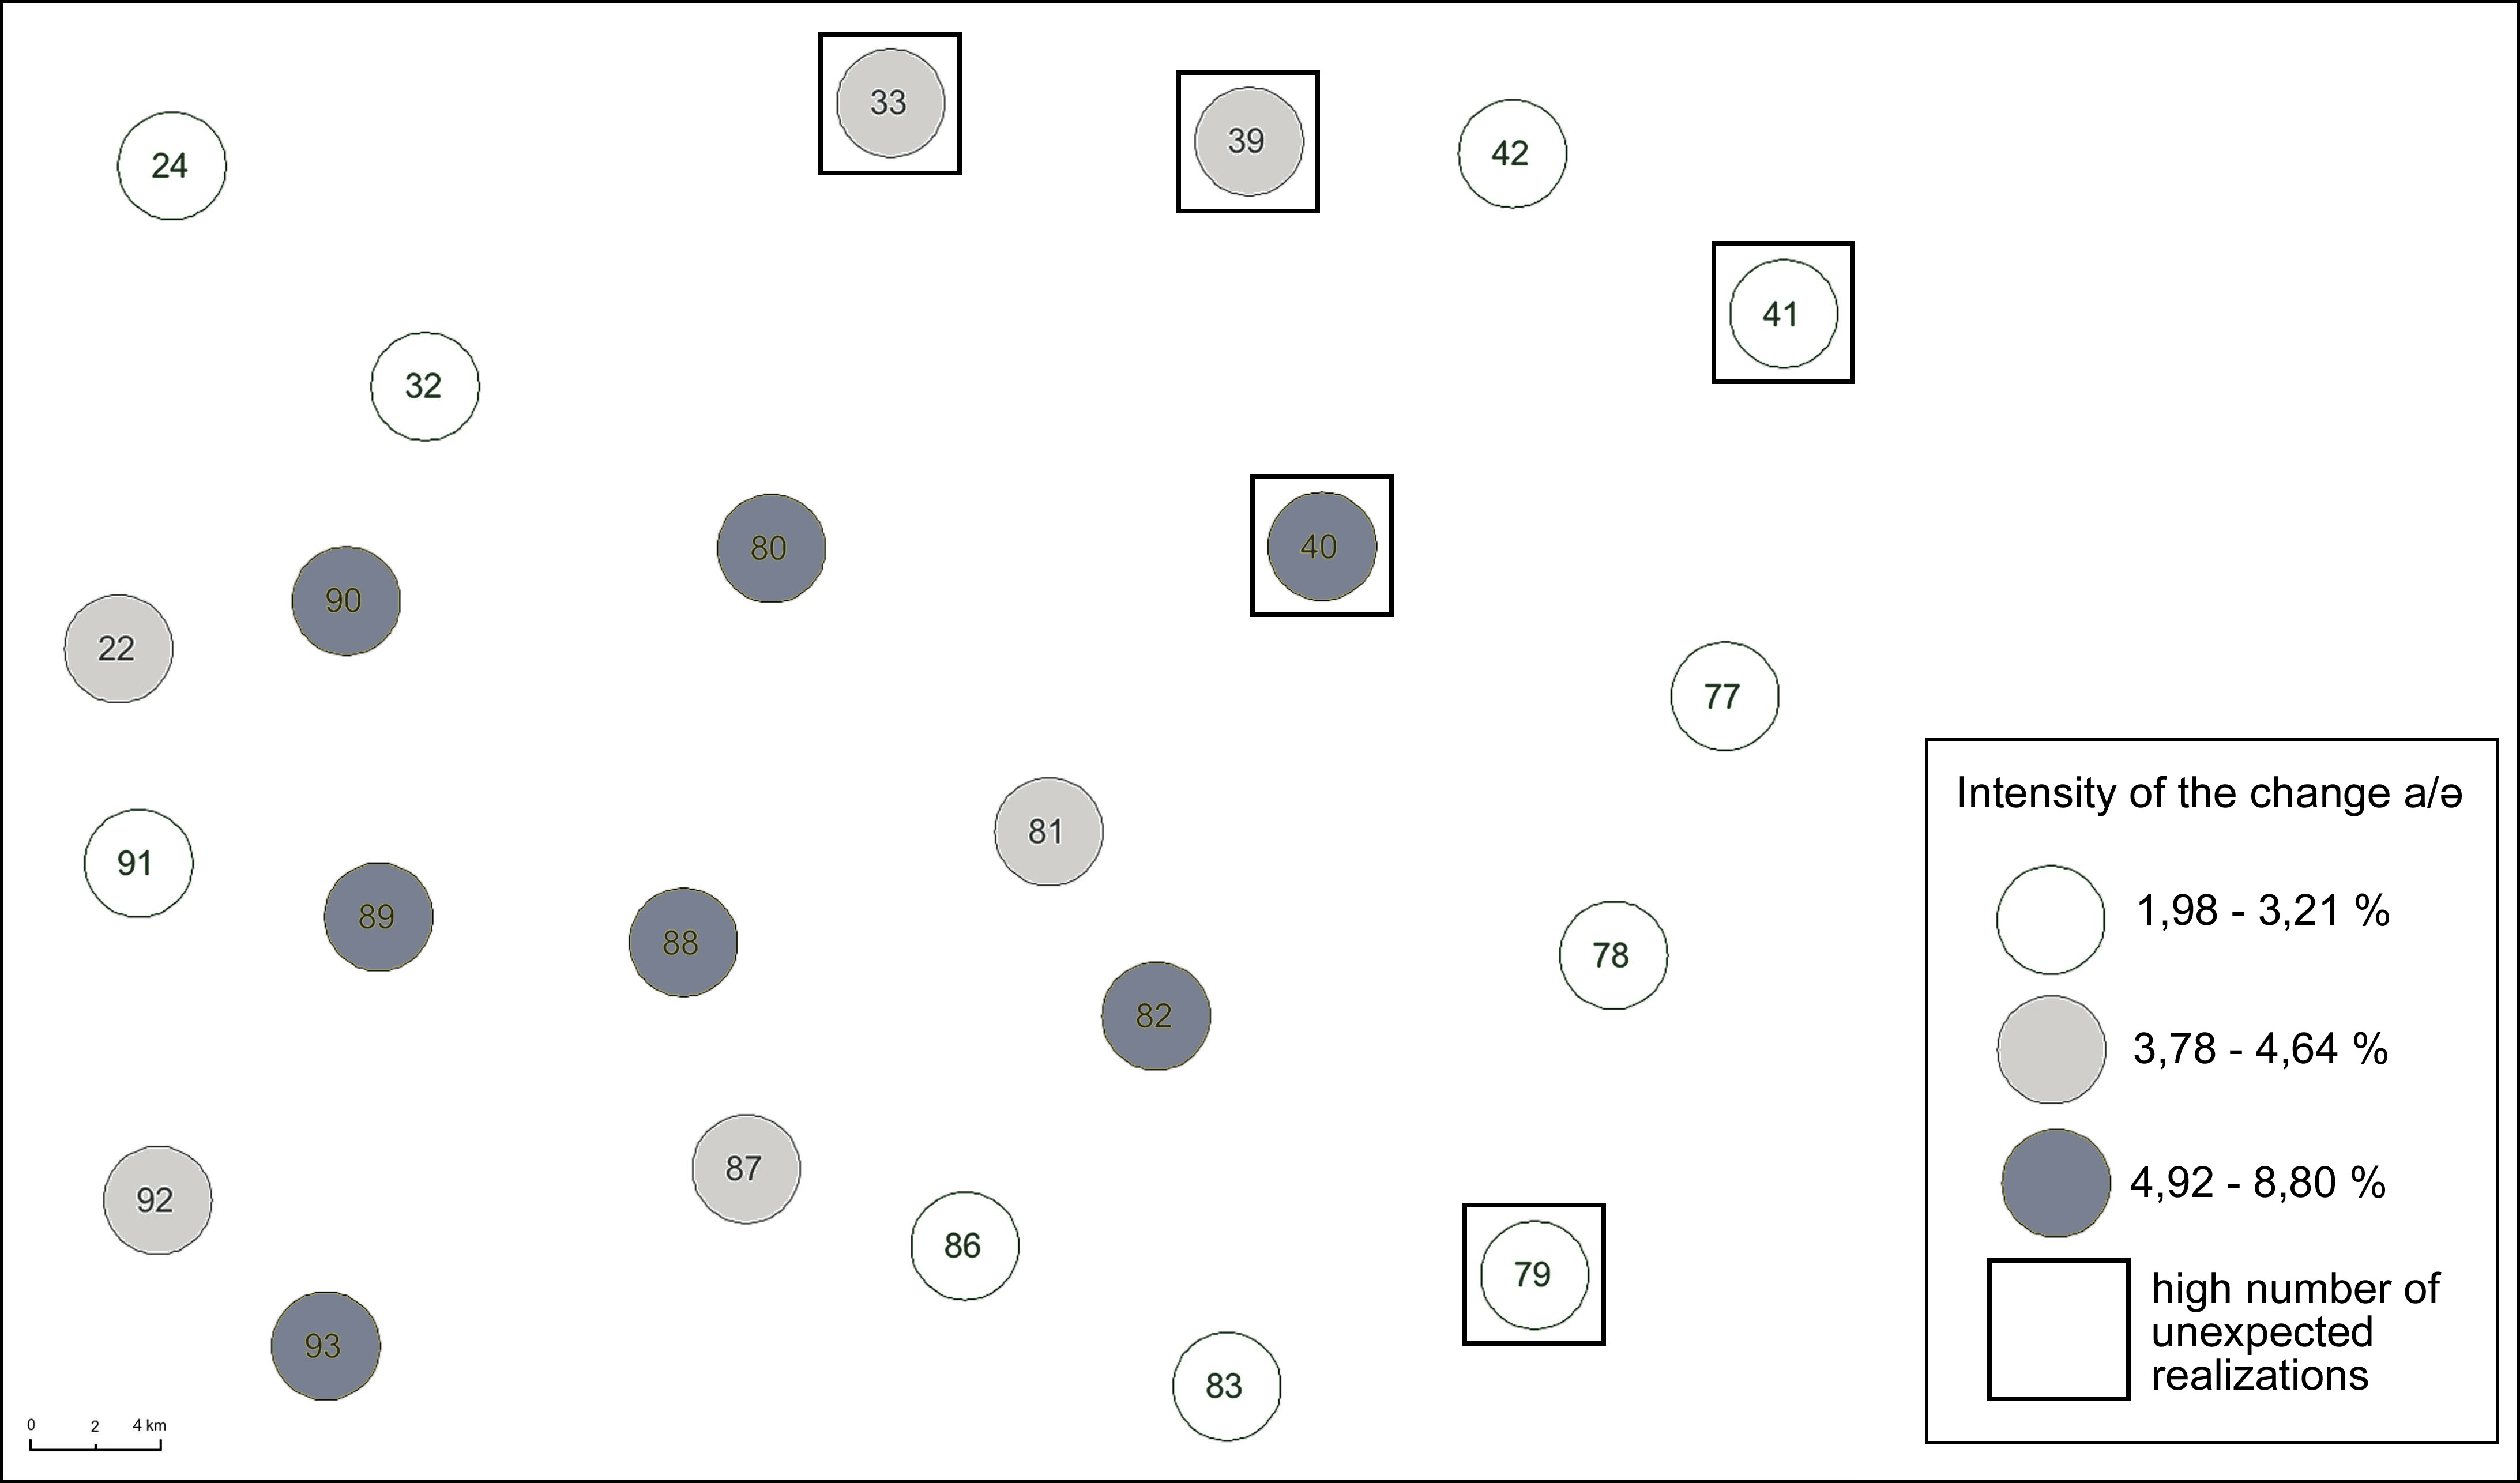
\includegraphics[width=\textwidth]{illustrations/brun_etal_fig6}
\caption{Intensity of the alternation ([a]/[ə]) across the area \& locations with a high number of specific realizations}
\label{fig:6}
\end{figure}

That kind of difference occurs the most intensely in the central area in dark grey. In the two other areas located on the fringes, the frequency is less important. At present, it is still difficult to draw a conclusion because we do not understand how this small area is connected to the rest of the Breton-speaking region, continuously or discontinuously.

Finally, a closer look at these results led us to identify a particular realization of the kind that occurs recurrently. Some words may end with an [a] and a final consonant (a+Cons.) in post-stressed contexts when a more common realization with a schwa and a final consonant (ə+Cons.) would have been expected as in the following example: NALBB map 109 ‘a day (long)’ point (33) Plougonven 'de̝:vas vs. point. (80) Berrien 'de̝:vəs.

This specific realization operates in a quite clear context especially in nouns and in the past participle forms of the verbs. This alternation cannot be explained by etymology. 

The realization of [a] for [ə] in final unstressed syllables occurs only in 45 cases in this category that is, 4.26\% of the total of the alternations ([a]/[ə]) and only 15 different lexemes in our corpus were affected by this specific realization. But it occurs in one little area and this specific realization is distributed as the following table shows:

\begin{table}
\resizebox{\textwidth}{!}{
\begin{tabular}{llll}
\lsptoprule
\begin{minipage}[t]{0.2\textwidth}Number of the point of enquiry \end{minipage} & 
\begin{minipage}[t]{0.2\textwidth}Location\end{minipage} & 
\begin{minipage}[t]{0.2\textwidth}Number of comparisons displaying the realization (a+Cons.)\end{minipage} & 
\begin{minipage}[t]{0.2\textwidth}Number of lexemes affected by the realization (a+Cons.)\end{minipage}\\
\midrule
 33 & {Plougonven} & 15 & 9\\
 40 & {Plourac’h} & 10 & 2\\
 41 & {Plougonver} & 4 & 2\\
 79 & {Paule} & 3 & 1\\
 88 & {Collorec} & 5 & 2\\
\lspbottomrule
\end{tabular}
}
\label{tab:7}
\caption{Distribution of the different occurrences of (a+Cons.) according to the location investigated}
\end{table}

This appears to be simply anecdotal on the surface but this specific realization regularly occurs in our corpus. Interestingly, the phenomenon is concentrated in the same micro-area around Plougonven (point 33). This means that this specific and not so common realization of a final unstressed (a+Cons.) could be salient from a sociolinguistic perspective as a sign of local identity and explain why an additional unneeded articulatory effort after the stressed syllable is produced for some words. Nevertheless, only a deeper scale study on these issues could help us to better understand the centralization of vowels in Breton.

\subsection[The differences around one locality]{The differences around one locality}

Another approach is a close examination of the data for one location in order to determine the phonetic similarity between neighbouring points. We decided to do this for Collorec (site 88), which is worth analysing because of its centrality and on account of the large number of results gathered for this place: 1354 alternations. They account for nearly 11\% of all the non-identical correspondences we observed in our corpus. This number is far higher than the average of changes for each locality (519) of the area. The following figures displayed the linguistic distance between Collorec and its closest neighbouring locations from a phonetic point of view.

\begin{table}
\resizebox{\textwidth}{!}{
\begin{tabular}{lll}
\lsptoprule
\begin{minipage}[t]{0.3\textwidth}{Site Comparison}\end{minipage} & 
\begin{minipage}[t]{0.3\textwidth}{Number of differences}\end{minipage} & 
\begin{minipage}[t]{0.3\textwidth}{Percentage compared to the number of differences}\end{minipage}\\
\midrule
{{88{\textgreater}90}} & {{293}} & {21.63}\\
{{82{\textgreater}88}} & {{256}} & {18.90}\\
{{80{\textgreater}88}} & {{246}} & {18.17}\\
{88{\textgreater}89} & {206} & {15.21}\\
{81{\textgreater}88} & {191} & {14.10}\\
{87{\textgreater}88} & {162} & {11.96}\\
\midrule
& {1354} & {99.97}\\
\lspbottomrule
\end{tabular}
}
\caption{Number of differences to neighbouring sites around Collorec (site 88)}
\label{tab:8}
\end{table}

\begin{figure}
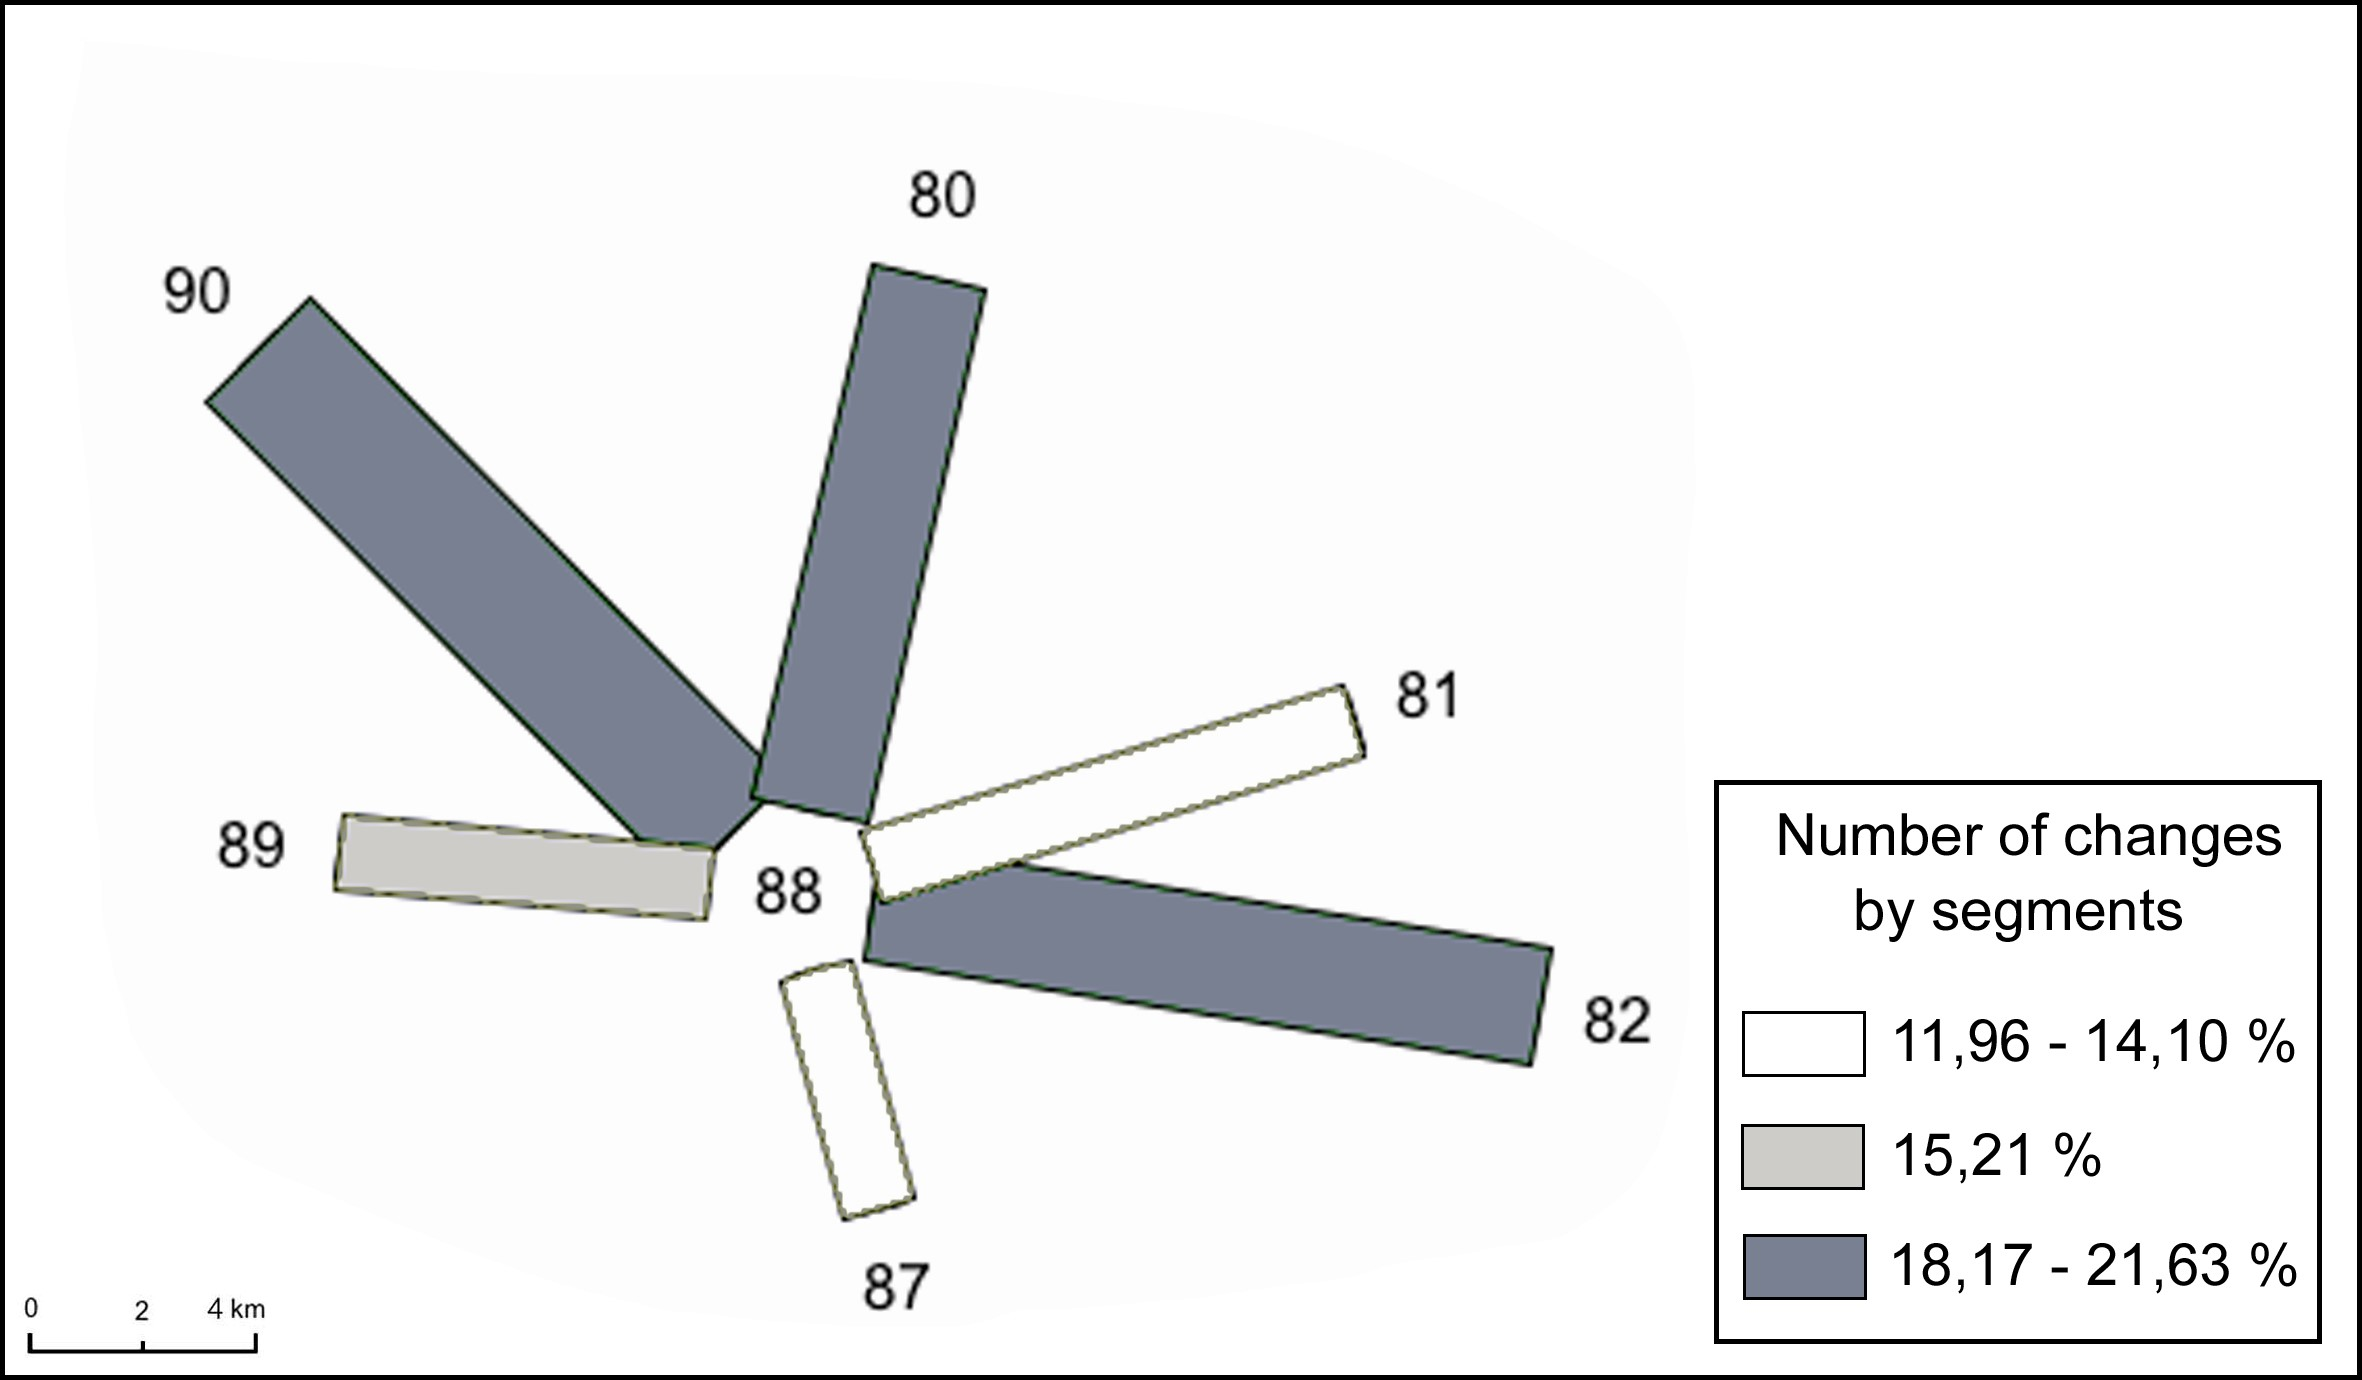
\includegraphics[width=\textwidth]{illustrations/brun_etal_fig7}
\caption{Number of differences to neighbouring sites around Collorec (point 88)}
\label{fig:7}
\end{figure}

\tabref{tab:8} shows how the differences observed between Collorec and its neighbouring points are represented spatially. For each segment the number of alternations we noticed corresponds to the average observed for all the other segments across the area (225 on average).

\figref{fig:7} shows that the level of intensity with respect to the differences varies according to the site-pair involved: three locations (80, 82, 90) are phonetically more distant from Collorec than the others. The distance we have noticed for sites 80 and 90 could be explained by a geographic factor: a bog named \textit{Yeun Ellez} spreads out between these points and Collorec. These findings about phonetic traits match Solliec’s own research in the area. This fen, which is an obstacle to circulation, seems to foster linguistic distance more than the hills (named \textit{Monts d’Arrée}), on the Northern-West edge of the area, which are easy to get over (see \figref{fig:3}: FuzzyMatch map).

Moreover, through the statistical use of the data returned by the DL algorithm, the features of the linguistic variation in Collorec can be examined. The alternations observed for Collorec are detailed in the following figures.

\begin{figure}
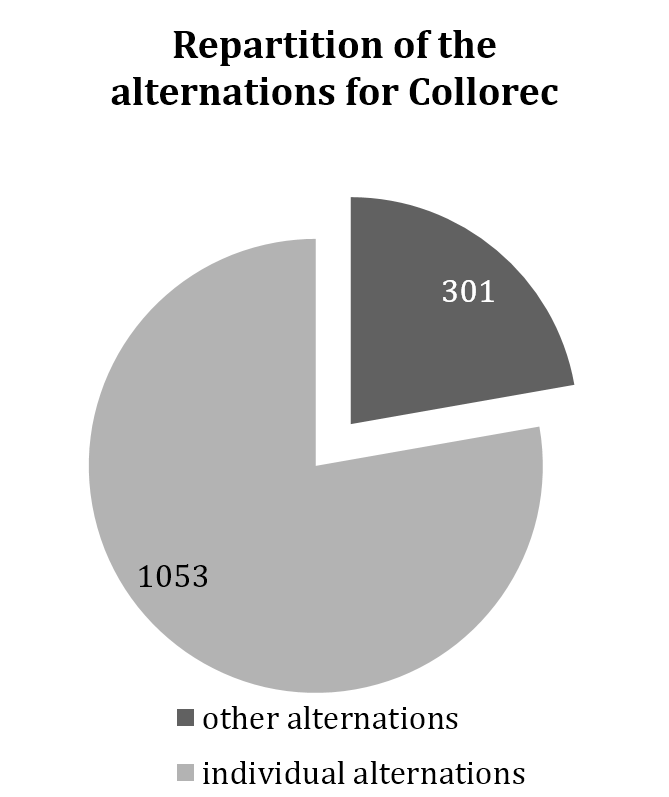
\includegraphics[width=0.5\textwidth]{illustrations/brun_etal_fig8}
\caption{Nature of the alternations between Collorec and its surrounding neighbours}
\label{fig:8}
\end{figure}

\begin{figure}
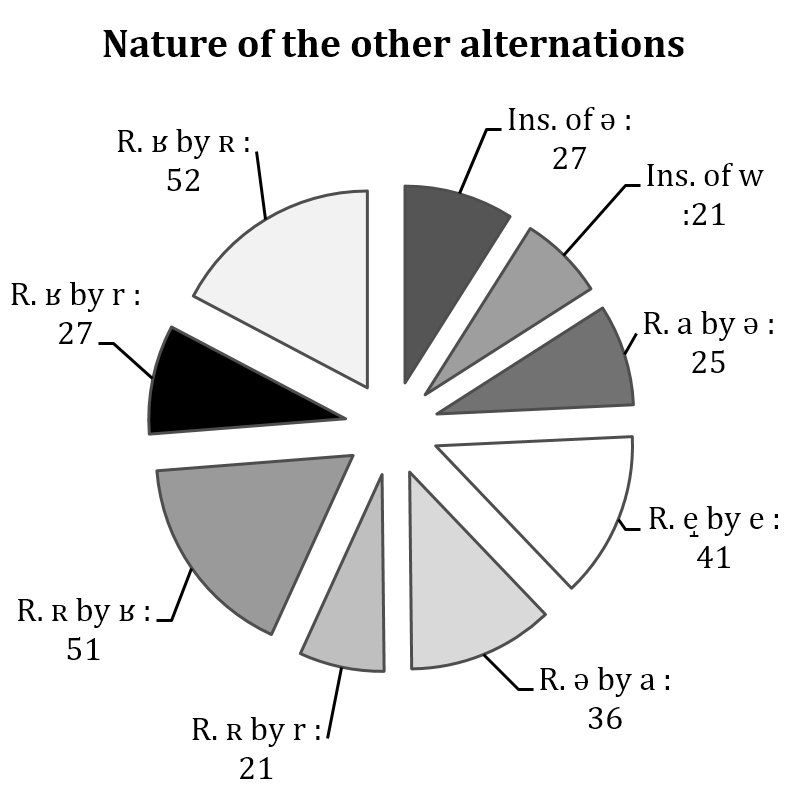
\includegraphics[width=0.5\textwidth]{illustrations/brun_etal_fig9}
\caption{Nature of the alternations between Collorec and its surrounding neighbours}
\label{fig:9}
\end{figure}

The diagrams 8 and 9 show how the non-identical phonetic correspondences we found between Collorec and the other surrounding locations are distributed. As these figures show, two types of alternations can be distinguished. The first one groups together the alternations thatonly show up once or twice in the results. In the second category are gathered the alternations, which can be clearly individualized (\figref{fig:9}) and which happen on a quite frequent basis.

These alternations are the same as those occurring across the whole area and with the same frequency, such as the different kinds of rhotics or the ([a]/[ə]) correspondence. Nevertheless, one must keep in mind that the number of occurrences for each alternation is low. For instance, 20 occurrences out of 1354 only account for 1.5\% of them. We didn’t find any alternation unique to Collorec in spite of the high amount of data we have at our disposal for this specific location, whose features thus share in the general tendencies of the area, which is quite uniform in phonetic terms.

These two different approaches, the first about a specific alternation and the second dealing with the phonetic features of one location are the type of investigation opportunities this new usage of the DL algorithm offers for geolinguistic research. 

\section{Conclusion}

To conclude, we want to stress that the sample of data used for this investigation was small because we deliberately restrained the size of the area under investigation as well as the amount of data. This paper reflects the first step of a more ambitious research to present a dialectometric analysis covering the whole Breton-speaking area. Our specific use of the DL algorithm allows us to treat qualitative data statistically. Linguistic variation can be described from a quantitative viewpoint while taking into account but the specific features at stake so as to present a more accurate view of the data under analysis.

Furthermore, this new method allows us to divide the results obtained into 3 main categories: vowels, consonants and rhotics. These categories will have to be analysed individually while keeping in mind they can interplay together. A further step to this research will be to elaborate a dialectometric analysis on a larger scale, based on the data of the NALBB, being conducted by Solliec as part of his PhD at the University of Brest in France. For this purpose, he will compare different dialectrometric techniques. The Breton-speaking area is interesting, as it constitutes a real linguistic laboratory thanks to its important inner variations and to its distinctiveness from the neighbouring romance varieties.

\section*{Acknowledgement}
We would like to thank Professor Gary German (UBO Brest) for his precious help in rereading and revising this paper.

\printbibliography[heading=subbibliography,notkeyword=this]
\end{document}
